\documentclass[aps,prd,amsfonts,amssymb,amsmath,nofootinbib,showpacs,superscriptaddress,twocolumn]{revtex4}
\usepackage{graphicx}
\usepackage{color}
%\usepackage{psfrag}
\usepackage{mathrsfs}
\usepackage{dcolumn}
\usepackage{hyperref}

\newcommand{\eqnref}[1]{(\ref{eq:#1})}
\newcommand{\figref}[1]{Fig.\ \ref{fig:#1}}
\newcommand{\Figref}[1]{Fig.\ \ref{fig:#1}}
\newcommand{\secref}[1]{Sec.\ \ref{sec:#1}}
\newcommand{\apref}[1]{Appendix \ref{sec:#1}}
\newcommand{\Tabref}[1]{Table \ref{tab:#1}}

\newcommand{\units}[1]{\ensuremath{~\mathrm{#1}}}

\newcommand{\sub}[1]{\ensuremath{_\text{#1}}}
\newcommand{\super}[1]{\ensuremath{^\text{#1}}}
\newcommand{\dd}{\ensuremath{\mathrm{d}}}
\newcommand{\diff}[2]{\ensuremath{\dfrac{\dd {#1}}{\dd {#2}}}}
\newcommand{\linediff}[2]{\ensuremath{\dd {#1}/\dd {#2}}}
\newcommand{\diffop}[1]{\ensuremath{\dfrac{\dd}{\dd {#1}}}}
\newcommand{\difftwo}[2]{\ensuremath{\dfrac{\dd^2 {#1}}{\dd {#2}^2}}}
\newcommand{\linedifftwo}[2]{\ensuremath{\dd^2 {#1}/\dd {#2}^2}}
\newcommand{\difftwoop}[1]{\ensuremath{\dfrac{\dd^2}{\dd {#1}^2}}}
\newcommand{\diffn}[3]{\ensuremath{\dfrac{\dd^{#3} {#1}}{\dd {#2}^{#3}}}}
\newcommand{\linediffn}[3]{\ensuremath{\dd^{#3} {#1}/\dd {#2}^{#3}}}
\newcommand{\diffnop}[2]{\ensuremath{\dfrac{\dd^{#2}}{\dd {#1}^{#2}}}}
\newcommand{\partialdiff}[2]{\ensuremath{\dfrac{\partial {#1}}{\partial {#2}}}}
\newcommand{\linepartialdiff}[2]{\ensuremath{\partial {#1}/\partial {#2}}}
\newcommand{\partialdiffop}[1]{\ensuremath{\dfrac{\partial}{\partial {#1}}}}\newcommand{\recip}[1]{\ensuremath{\frac{1}{#1}}}
\newcommand{\grad}{\ensuremath{\boldsymbol{\nabla}}}
\newcommand{\intd}[4]{\ensuremath{\int_{#1}^{#2}{#3}\,\dd{#4}}}
\newcommand{\order}[1]{\ensuremath{\mathcal{O}({#1})}}

\newcommand{\overlap}[2]{\ensuremath{\left(#1\middle|#2\right)}}

\DeclareMathOperator{\sgn}{sgn}

\begin{document}

%\preprint{}

\title{The importance of transient resonances in extreme-mass-ratio inspirals (new title?)}

\author{Robert H. Cole}
\email[]{rhc26@ast.cam.ac.uk}
\affiliation{Institute of Astronomy, Madingley Road, Cambridge, CB3 0HA, United Kingdom}
\author{Christopher P.L. Berry}
\email[]{cplb@star.sr.bham.ac.uk}
\affiliation{School of Physics and Astronomy, University of Birmingham, Edgbaston, Birmingham B15 2TT, United Kingdom}
\affiliation{Institute of Astronomy, Madingley Road, Cambridge, CB3 0HA, United Kingdom}
\author{Priscilla Ca\~{n}izares}
\email[]{pcm@ast.cam.ac.uk}
\author{Jonathan R. Gair}
\email[]{jgair@ast.cam.ac.uk}
\affiliation{Institute of Astronomy, Madingley Road, Cambridge, CB3 0HA, United Kingdom}

\date{\today}

\begin{abstract}
\emph{Update abstract}
The inspiral of stellar-mass compact objects into supermassive black holes provides a wealth of information about the strong gravitational-field regime via the emission of gravitational waves. In order to detect such signals and extract the desired information, it is necessary to possess a bank of accurate waveform templates. For computational efficiency, adiabatic templates are often used, which accurately reproduce orbit-averaged trajectories arising from the first order dissipative gravitational self-force. Other effects are however neglected, in particular that of transient resonances, where the radial and poloidal fundamental frequencies become commensurate. During such resonances, the flux of gravitational waves can be diminished or enhanced, leading to a shift in the compact-object trajectory and, ultimately, the phase of the emitted radiation. In this work, an astrophysical population of detectable extreme-mass-ratio inspirals is studied and it is found that a large proportion shall encounter a low-order resonance in the later stages of inspiral. The resulting effect on signal-to-noise recovery is small due to the low eccentricity of the studied population, but nevertheless at least one fifth of the systems may become undetectable if transient resonances are not accounted for.
\end{abstract}

% 04.25.Nx 	Post-Newtonian approximation; perturbation theory; related approximations
% 04.30.-w 	Gravitational waves
% 04.70.-s 	Physics of black holes
% 98.62.Js 	Galactic nuclei (including black holes), circumnuclear matter, and bulges 
\pacs{04.25.Nx, 04.30.--w, 04.70.--s, 98.62.Js}

\maketitle

\section{Introduction}

In the prologue to his classic monograph, Chandrasekhar~\cite{Chandrasekhar1992} celebrates the simplicity of black holes (BHs). The Kerr solution is defined by just two parameters: mass and spin. Despite the baldness of the BH metrics, great intricacies manifest in their properties. This is made evident when a second body is introduced. The two-body problem in general relativity (GR) is well studied. It is of paramount importance for gravitational-wave (GW) astronomy, where binary systems are the dominant source of radiation. Correctly modelling the dynamics of these systems is necessary to interpret and extract information from gravitational waveforms.

We have made progress in understanding the general relativistic two-body problem in recent years. Bodies of comparable mass can be studied using numerical relativity. Rapid advances in this field have been made following breakthroughs in 2005~\cite{Pretorius2005,Campanelli2006,Baker2006}. These simulations shall allow us to understand BH--BH mergers. Stellar-mass BH mergers are targets for ground-based GW detectors, such as the currently mid-upgrade LIGO~\cite{Harry2010} and Virgo~\cite{Accadia2011}, and the in-construction KAGRA~\cite{Kuroda2010}. Massive BH mergers, expected to be the result of galaxy mergers, are potential sources for a space-borne detector such as eLISA~\cite{Amaro-Seoane2012a}. Systems of unequal masses are more challenging to evolve numerically as they complete a larger number of orbits and it is necessary to resolve two different scales. Calculations can instead be performed perturbatively. The paradigm unequal-mass system has a stellar-mass BH orbiting a massive black hole, such as those expected to be found at the centre of most galaxies. These extreme-mass-ratio inspirals (EMRIs) produce GWs that are a promising signal for space-borne detectors~\cite{Amaro-Seoane2007}. Despite being well-studied there still remain open questions.

In the case of extreme-mass-ratio systems, efforts are concentrated on understanding the gravitational self-force~\cite{Barack2009,Poisson2004}. In the test particle limit, the smaller body follows an exact geodesic of the BH's spacetime. Including the effects of the smaller body's finite mass, the background spacetime is perturbed. The back-reaction from this deformation alters the small body's orbital trajectory, and can be modelled as a self-force that moves the body from its geodesic. The self-force is commonly divided into two pieces, dissipative and conservative. The former encapsulates the slow decay of the orbital energy and angular momentum, constants of the motion in the test particle limit, through radiation. The latter shifts the orbital phases inducing precession. The dissipative piece is time-asymmetric and has the larger effect on the evolution of the orbital phase; the conservative piece is time-symmetric and has a smaller influence on the phase although this can accumulate over many orbits. Being able to accurately model the influence of the self-force shall allow us to create reliable waveform models.

Flanagan and Hinderer~\cite{Flanagan2012} highlighted a previously overlooked phenomenon that occurs in the general relativistic two-body problem, that of transient resonances. Geodesic orbits in GR have three associated frequencies: the radial frequency $\Omega_r$, the polar frequency $\Omega_\theta$ and the azimuthal frequency $\Omega_\phi$. The first two describe libration and the third rotation (except in the case of polar orbits where $\Omega_\theta$ also describes rotation)~\cite{Goldstein2002}. % Section 10.6
In the weak-field limit, these all tend towards the Keplerian frequency; in the strong-field, $\Omega_r < \Omega_\theta < \Omega_\phi$, and they may differ significantly. For extreme-mass-ratio systems, the evolution time-scale is much longer than the orbital period such that the motion of the smaller body is approximately geodesic over orbital time-scales. The evolution of the orbit can be approximated as a series of geodesics using the osculating element formalism~\cite{Pound2008,Gair2011a}. During this evolution, the frequencies may become commensurate. Resonances occur when the radial and polar frequencies are rational multiples of each other:
\begin{equation}
\nu = \frac{\Omega_r}{\Omega_\theta} = \frac{n_\theta}{n_r},
\end{equation}
where $n_r$ and $n_\theta$ are integers (with no common factors). During resonance, terms in the self-force that usually average to zero can combine coherently, significantly impacting the orbital motion~\cite{Flanagan2012a}. Resonances involving the azimuthal motion do not produce a comparable effect because of the axisymmetry of the background spacetime.

Geodesic motion in Kerr spacetime can be described by use of the action--angle formalism~\cite{Goldstein2002}. % Chapter 10
We consider a body of mass $\mu$ orbiting a BH of mass $M$, with $\eta = \mu/M \ll 1$,\footnote{To first order, the mass ratio $\eta$ is the same as the symmetric mass ratio $\mu M/(\mu+M)^2$.} and describe the motion in the directions of the standard Boyer--Lindquist coordinates $\{t,r,\theta,\phi\}$ using generalised angle variables $q_\alpha = \{q_t,q_r,q_\theta,q_\phi\}$ \citep{Hinderer2008}. We denote the first integrals of the geodesic motion, the generalised action variables, by $J_\alpha$. These are some combination of the energy per unit mass $E$ and the axial angular momentum per unit mass $L_z$, which arise from isometries of the metric in $t$ and $\phi$, and the Carter constant per unit mass squared $Q$~\cite{Carter1968}, which is related to the separability of the equations of motion in $r$ and $\theta$. The system evolves following~\cite{Flanagan2012}
\begin{subequations}
\label{eq:Mino-E-o-M}
\begin{align}
\diff{q_\alpha}{\lambda} = {} & \omega_\alpha(\boldsymbol{J}) + \eta g_\alpha^{(1)}(q_r,q_\theta,\boldsymbol{J}) + \order{\eta^2}, \\
\diff{J_\alpha}{\lambda} = {} & \eta G_\alpha^{(1)}(q_r,q_\theta,\boldsymbol{J}) + \order{\eta^2},
\end{align}
\end{subequations}
where $\lambda$ is Mino time~\cite{Mino2003}, and the forcing functions $g_\alpha^{(1)}$ and $G_A^{(1)}$ originate from the first-order self-force. By working with $\lambda$ instead of proper time $\tau$, the radial and polar motions decouple. At zeroth order in the mass ratio we recover the limit of purely geodesic motion: the integrals of the motion are actually constants and the angle variables evolve according to their associated frequencies $\omega_\alpha$.

The leading order dissipative correction to geodesic motion is calculated following the adiabatic prescription~\cite{Hinderer2008}: by dropping the forcing term $g_\alpha^{(1)}$ (and all higher order terms) and replacing the forcing term $G_\alpha^{(1)}$ with its average over the $2$-torus parametrized by $q_r$ and $q_\theta$ $\langle G_\alpha^{(1)}\rangle_{q_r,\,q_\theta}$~\cite{Drasco2005}. For most orbits this is sufficient, $G_\alpha^{(1)}$ is given by its average value plus a rapidly oscillating component~\cite{Arnold1988}. % Chapter 5, section 1
However, this averaging fails when the ratio of frequencies is the ratio of integers. In this case the trajectory does not ergodically fill the $2$-torus, but instead traces out a $1$-dimensional subspace.\footnote{For illustrations, see Grossman, Levin and Perez-Giz~\cite{Grossman2012}.} There are then contributions to the self-force that no longer average out beyond $\langle G_A^{(1)}\rangle_{q_r,\,q_\theta}$. Intuitively, we expect that this effect is more important for ratios of small integers as when the integers are large, the orbit comes close to all points on the $2$-torus.

In this work we seek to characterise the importance of these resonances for the purposes of modelling EMRIs. The amplitude of expected signals shall be below the level of noise in a space-based GW detector. However, systems remain in band for many hundreds of thousands of cycles and so may be detected using a matched filter, provided we have sufficiently accurate waveform templates. Ensuring the accuracy of EMRI templates requires calculating the impact that passing through a resonance has on the orbital evolution and discovering for which resonances this is significant.

In \secref{problem}, we formulate the specific problem at hand: that of geodesic motion in Kerr spacetime, perturbed by the gravitational self-force. We then study generic properties of transient resonances in \secref{properties}, detailing their location in parameter space, the time-scales over which they affect the motion and the resulting GW flux enhancements. Specific examples are considered to illustrate the effects of resonances at the start of \secref{astrophysics}, before finally turning to an astrophysical population in \secref{population}. Our conclusions can be found in \secref{conclusion}.

We use geometric units with $G = c = 1$ throughout. We always use $M$ for the mass of the central massive BH and $a$ as the spin parameter. We also use the dimensionless spin $a_\ast \equiv a/M$; we take the convention that $0 \leq a_\ast < 1$.

\section{Problem formulation}
\label{sec:problem}
\subsection{Kerr geodesics}

The evolution of an extreme-mass-ratio ($\eta \ll 1$) system is slow. Instantaneously, the motion of the orbiting mass can be described as geodesic, with the integrals of the motion changing on time-scales of many orbital periods. We analyse the behaviour of resonances within the osculating element framework, where the trajectory is described by a sequence of geodesics that each match onto the motion at a particular instance. It is therefore necessary to develop an understanding of the Kerr geodesics.

The geodesic equations may be written as~\cite{Carter1968, Chandrasekhar1992} % section 62
\begin{subequations}
\begin{align}
\diff{t}{\lambda} = {} & a\left(L_z - aE\sin^2 \theta\right) + \frac{r^2 + a^2}{\Delta}\mathcal{T},\\
\diff{r}{\lambda} = {} & \pm \sqrt{V_r},\\
\diff{\theta}{\lambda} = {} & \pm \sqrt{V_\theta},\\
\diff{\phi}{\lambda} = {} & \frac{L_z}{\sin^2 \theta} - aE + \frac{a}{\Delta}\mathcal{T},
\end{align}
\end{subequations}
where $\Delta = r^2 - 2M r + a^2$; the signs of the $r$ and $\theta$ equations can be chosen independently, and we have introduced potentials
\begin{subequations}
\begin{align}
\mathcal{T} = {} & E\left(r^2 +a^2\right) - aL_z,\\
V_r = {} & \mathcal{T}^2 - \Delta\left[r^2 + \left(L_z -aE\right)^2 + Q\right],\\
V_\theta = {} & Q - \cos^2 \theta\left[a^2\left(1 - E^2\right) + {\displaystyle \frac{L_z^2}{\sin^2\theta}}\right].
\end{align}
\end{subequations}
As an affine parameter, we have used Mino time which is related to the proper time $\tau$ by~\cite{Mino2003}
\begin{equation}
\tau = \intd{}{}{r^2 + a^2 \cos^2\theta}{\lambda}.
\end{equation}
Using Mino time allows us to decouple the $r$ and $\theta$ motions.

We only consider bound motion~\cite{Wilkins1972}: the radial motion covers a range $r\sub{p} \leq r \leq r\sub{a}$, where the turning points are the periapsis $r\sub{p}$ and apoapsis $r\sub{a}$. Drawing upon Keplerian orbits we parametrize the motion using
\begin{equation}
r = \frac{p M}{1+e\cos\psi},
\end{equation}
introducing eccentricity $e$, (dimensionless) semilatus rectum $p$ and relativistic anomaly $\psi$~\cite{Darwin1961,Drasco2004}. While $r$ oscillates between its maximum and minimum values, $\psi$ increases secularly, increasing by $2\pi$ across an orbit. The polar motion covers a range $\theta_- \leq \theta \leq \pi - \theta_-$. We also parametrize this motion in terms of an angular phase $\chi$, according to~\cite{Hughes2000}
\begin{equation}
\cos\theta = \cos\theta_-\cos\chi.
\end{equation}
While $\psi$ and $\chi$ are $2\pi$ periodic they are not the canonical action--angle variables~\cite{Schmidt2002}; they are, however, easy to work with.

The geodesic motion can equally be described by $\{E,L_z,Q\}$ or $\{p,e,\theta_-\}$~\cite{Schmidt2002}. Converting between them requires finding the solutions of $V_r = 0$ and $V_\theta = 0$. We employ a slightly different parameter set of $\{p,e,\iota\}$ where we have introduced the inclination~\cite{Ryan1996,Glampedakis2002}
\begin{equation}
\tan \iota = \frac{\sqrt{Q}}{L_z}.
\end{equation}
This is $0 \leq \iota < \pi/2$ for prograde orbits and $\pi/2 < \iota \leq \pi$ for retrograde orbits. Equatorial orbits ($\theta_- = \pi/2$) have $\iota = 0$ or $\pi$ and polar orbits ($\theta_- = 0$) have $\iota = \pi/2$. While formulae exist for conversion between the different parameters, these are complicated and uninsightful, so we do not reproduce them here.\footnote{In practice we find turning points numerically.}

\subsection{Orbital resonances}

The radial and polar orbital periods in Mino time are given by
\begin{subequations}
\begin{align}
\Lambda_r = {} & 2\intd{r\sub{p}}{r\sub{a}}{\recip{\sqrt{V_r}}}{r} = \intd{-\pi}{\pi}{\diff{\lambda}{\psi}}{\psi}, \\
\Lambda_\theta = {} & 4\intd{\theta_-}{\pi/2}{\recip{\sqrt{V_\theta}}}{\theta} = \intd{-\pi}{\pi}{\diff{\lambda}{\chi}}{\chi}.
\end{align}
\end{subequations}
The orbital frequencies are thus
\begin{equation}
\Upsilon_r = \frac{2\pi}{\Lambda_r}, \quad \Upsilon_\theta = \frac{2\pi}{\Lambda_\theta}.
\end{equation}
The geodesic equations for coordinate time $t$ and azimuthal angle $\phi$ are just functions of $r$ and $\theta$, hence their evolutions can be expressed as Fourier series~\cite{Drasco2004}
\begin{subequations}
\begin{align}
\diff{t}{\lambda} = {} & \sum_{k_r,\,k_\theta}T_{k_r,\, k_\theta}\exp\left[-i\left(k_r\Upsilon_r + k_\theta\Upsilon_\theta\right)\lambda\right], \\
\diff{\phi}{\lambda} = {} & \sum_{k_r,\,k_\theta}\Phi_{k_r,\, k_\theta}\exp\left[-i\left(k_r\Upsilon_r + k_\theta\Upsilon_\theta\right)\lambda\right].
\label{eq:Mino-Fourier}
\end{align}
\end{subequations}
The $(0,\,0)$ coefficients in these series give the average secular rate of increase of these quantities. We define
\begin{equation}
\Gamma = T_{0,\,0}, \quad \Upsilon_\phi = \Phi_{0,\,0}
\end{equation}
to act as Mino-time frequencies. We can now convert to coordinate-time frequencies with
\begin{equation}
\Omega_r = \frac{\Upsilon_r}{\Gamma}, \quad \Omega_\theta = \frac{\Upsilon_\theta}{\Gamma}, \quad \Omega_\phi = \frac{\Upsilon_\phi}{\Gamma}.
\end{equation}

Transient resonances occur when the radial and poloidal motions are commensurate, when
\begin{equation}
\nu = \frac{\Upsilon_r}{\Upsilon_\theta} = \frac{\Omega_r}{\Omega_\theta} = \frac{n_\theta}{n_r}
\end{equation}
is the ratio of small integers. At this point, any Fourier series like those in \eqnref{Mino-Fourier} goes from being an expansion in two frequencies to being an expansion in a single frequency~\cite{Bosley1992}.

For a general non-resonant orbit there is no fixed correlation between the radial and polar coordinates. After a sufficiently long time, the trajectory comes arbitrarily close to every point in the range of motion (with $r\sub{p} \leq r \leq r\sub{a}$ and $\theta_- \leq \theta \leq \pi - \theta_-$); on account of the orbital precession, the whole space is densely covered. This does not happen on resonance, as the radial and polar motions are locked together such that we can express one as a function of the other, and so the trajectory keeps cycling over the same path. The points visited are controlled by the relative phases of the $r$ and $\theta$ motions. To represent this, we use the $r$ phase at the $\theta$ turning point $\psi_{\theta_-} = \psi(\chi = 0)$. Varying $\psi_{\theta_-}$ across its full range allows every point in the range of motion to be reached. Hence averaging over all values of $\psi_{\theta_-}$ for resonant orbits is equivalent to averaging over the $\psi$--$\chi$ $2$-torus for non-resonant orbits.

One might be concerned about the nature of resonances following the inclusion of the self-force: true geodesic motion only exists at zeroth order in $\eta$ and, while it is a good approximation over short time-scales, for small $\eta$ there is a small disparity. The conservative piece of the self-force induces extra precession which leads to a slight shift in the orbital frequencies~\cite{Warburton2012}.\footnote{The Kolmogorov--Arnold--Moser (KAM) theorem states that when an integrable Hamiltonian (i.e., the case for motion in Kerr) is subject to a small perturbation the form of the orbits is preserved albeit slightly deformed~\cite{Arnold1963,Moser1973}. % Chapter II, section 3.3 d)
This should ensure that, in general, there are only small shifts in the orbital frequencies. However, the KAM theory only applies for sufficiently incommensurate orbits: close to resonance it does not apply~\cite{Moser1973}. % Chapter V section 1. c) 
This is a further reason why resonances merit an in-depth investigation.}
The dissipative piece causes the frequencies to evolve and, hence, the resonance cannot persist for multiple orbits (without some feedback coupling). In effect, we are really considering a period of time about the resonant crossing. The instantaneous orbital frequencies oscillate back and forth around their averaged values.

However, there shall be a time span when the frequencies are consistently close to being commensurate. During this time, the trajectory appears similar to a resonant trajectory, filling only a smaller region of the parameter space. It is this time period that is of interest for transient resonances~\cite{Bosley1992}.

%The Kolmogorov--Arnold--Moser (KAM) theorem states that when an integrable Hamiltonian (i.e., the case for motion in Kerr) is subject to a small perturbation the form of the orbits are preserved albeit slightly deformed~\cite{Arnold1963,Moser1973}. % Chapter II, section 3.3 d)
%When we average the self-force and follow the adiabatic evolution of the trajectory we are exploiting this behaviour. However, the KAM theory only applies for sufficiently incommensurate orbits: close to resonance it does not apply~\cite{Moser1973}. % Chapter V section 1. c)
% In these regions the adiabatic approximation breaks down and we need to follow the instantaneous evolution.


\subsection{Forced motion}
\label{sec:forced-motion}

For generic EMRIs, there are two timescales of interest: the \emph{fast} orbital motion, related to the fundamental frequencies $\sim1/\Omega$, and the \emph{slow} inspiral, related to the change in fundamental frequencies $\sim\Omega/\dot{\Omega}$, where an overdot denotes a derivative with respect to coordinate time $t$. These, along with the resonance timescale, are discussed more in \secref{res-time}. The two-timescale nature of the problem makes it ideally suited to the method of osculating elements~\cite{Gair2011a}: on short timescales, we analyse the unperturbed system resulting in geodesic motion, and then the long-term evolution is described by a sequence of instantaneous geodesics.

We require, at each instant in time, that the chosen geodesic matches the true position and velocity of the particle. This amounts to a specific choice of the orbital shape parameters (for example, the set $\{E,L_z,Q\}$ or the generalised action variables $J_\alpha$) and some initial phases at $t=t_0$ (for example, the set $\{\psi_0,\chi_0,\phi_0\}$). Collectively, these are referred to as \emph{osculating elements} and we denote them by $I^A(t)$, making explicit the variation with time.

Given geodesic motion in some background spacetime with Christoffel symbols $\Gamma^\alpha_{\beta\gamma}$, forced by some external acceleration $f^\alpha$, so that
\begin{equation}
\difftwo{x^\alpha}{\tau} + \Gamma^\alpha_{\beta\gamma}\diff{x^\beta}{\tau}\diff{x^\gamma}{\tau} = f^\alpha,
\end{equation}
we can calculate the evolution of the osculating elements $\dot{I}^A$. The specific equations for motion in Kerr are derived by Gair {\it{et al}}.~\cite{Gair2011a}.


\subsection{Self-force model}
\label{sec:self-force}

To follow the evolution of the inspiral we must have a means of prescribing the forcing acceleration. In this work we choose to work directly with the gravitational self-force, using the same post-Newtonian (PN) approximation as Flanagan and Hinderer~\cite{Flanagan2012}. For comparison, Flanagan, Hughes and Ruangeri~\cite{Flanagan2012a} use a Teukolsky equation calculation of GW fluxes to account for the inspiral due to radiation reaction.

The self-force model uses the first-order PN terms of the dissipative self-force formulated in Flanagan and Hinderer~\cite{Flanagan2007} and the conservative force formulated in Iyer and Will~\cite{Iyer1993}, and Kidder~\cite{Kidder1995}. Since only the first PN terms are used, this prescription can only be of limited validity in strong fields. Both pieces of the self-force are computed assuming that the spin is small: the dissipative piece contains terms to $\order{a_\ast^2}$ and the conservative piece to $\order{a_\ast}$. This is less than ideal for high spins. While this approximate self-force is not perfect, it should serve as a guide for the behaviour of the full self-force, allowing us to assess the qualitative impact of resonances on EMRI detection.

\emph{Add detail about why self-force model is rubbish. Comment on switching conservative piece off for population results.}

\subsection{Adiabatic evolution}
\label{sec:adiabatic}

Beyond geodesic motion in the Kerr spacetime, a test particle follows an accelerated trajectory determined by \eqnref{Mino-E-o-M}. This may be approximated by the adiabatic prescription~\cite{Hinderer2008} by dropping the forcing term $g_\alpha^{(1)}$ (and all higher-order terms) and replacing $G_\alpha^{(1)}$ with its average over the $2$-torus parametrized by $q_r$ and $q_\theta$, $\langle G_\alpha^{(1)}\rangle_{q_r,\,q_\theta}$~\cite{Drasco2005}. This piece is purely dissipative and determines how the inspiral evolves due to the radiation of GWs.

To construct an adiabatic trajectory we need the $2$-torus-averaged fluxes of our osculating elements. Computing an average of a quantity over the $\{q_r, q_\theta\}$ is trivial if it is parametrized in terms of these variables,
\begin{equation}
\left\langle \diff{X}{\lambda}\right\rangle_{q_r,\,q_\theta} = \frac{1}{(2\pi)^2}\intd{0}{2\pi}{\intd{0}{2\pi}{\diff{X}{\lambda}}{q_r}}{q_\theta}.
\end{equation}
However, we are using $\psi$ and $\chi$, as these are simpler to evolve; furthermore, we compute instantaneous co-ordinate time fluxes $\dot{X}$, not Mino-time fluxes. Changing variables gives an average of \cite{Drasco2005}
\begin{widetext}\begin{align}
\left\langle \diff{X}{\lambda}\right\rangle_{q_r,\,q_\theta} = {} & \frac{1}{\Lambda_r \Lambda_\theta}\intd{0}{2\pi}{\intd{0}{2\pi}{\left(\diff{\psi}{t}\right)^{-1} \left(\diff{\chi}{t}\right)^{-1} \left(\diff{t}{\lambda}\right)^{-2} \diff{X}{\lambda}}{\psi}}{\chi} \\
 = {} & \frac{1}{\Lambda_r \Lambda_\theta}\intd{0}{2\pi}{\intd{0}{2\pi}{\left(\diff{\psi}{t}\right)^{-1} \left(\diff{\chi}{t}\right)^{-1} \left(\diff{t}{\lambda}\right)^{-1} \dot{X}}{\psi}}{\chi}.
\label{eq:2torus-average}
\end{align}\end{widetext}
This average describes the Mino-time rate of change of the quantity $X$ over an orbit. To convert to a co-ordinate flux of the averaged quantity, we simply divide by the period $\Gamma$, defining
\begin{equation}
\dot{\left\langle X\right\rangle}_{q_r,\,q_\theta} = \frac{1}{\Gamma}\left\langle \diff{X}{\lambda}\right\rangle_{q_r,\,q_\theta}.
\end{equation}
Is in convenient to calculate $\Gamma$ as
\begin{equation}
\Gamma = \left\langle \diff{t}{\lambda}\right\rangle_{q_r,\,q_\theta},
\end{equation}
using \eqnref{2torus-average}, as this allows us to eliminate $\Lambda_r$ and $\Lambda_\theta$ from the calculation. The averaged fluxes successfully describe the leading-order secular evolution of the trajectory, as illustrated in \figref{good-traj}.

%In our parameterisation of the EMRI system, using $\{\psi,\chi\}$ rather than $\{q_r,q_\theta\}$, we must perform appropriate averages over this new $2$-torus. The osculating elements integration scheme involves computing derivatives with respect to coordinate time, and we shall often be interested in the averaged form of such derivatives. Given a function $X(\psi,\chi)$, we can calculate the 2-torus average \cite{Drasco2005} of the derivative with respect to Mino time in terms of precomputed quantities
%\begin{widetext}\begin{equation}
%\label{eq:2torus-average}
%\left\langle \diff{X}{\lambda}\right\rangle_{\psi,\,\chi} = \frac1{\Lambda_r\Lambda_\theta} \intd{0}{2\pi}{ \intd{0}{2\pi}{ \left(\diff{\psi}{t}\right)^{-1} \left(\diff{\chi}{t}\right)^{-1} \left(\diff{t}{\lambda}\right)^{-1} \dot{X} }{\chi} }{\psi}.
%\end{equation}\end{widetext}
%We then obtain a coordinate time derivative
%\begin{equation}
%\dot{\left\langle X\right\rangle}_{\psi,\,\chi} = \left.\left\langle \diff{X}{\lambda}\right\rangle_{\psi,\,\chi}\middle/\left\langle \diff{t}{\lambda}\right\rangle_{\psi,\,\chi}\right.,
%\end{equation}
%which is successful at describing the leading-order secular evolution of the trajectory, as illustrated in \figref{good-traj}.

\emph{Remove from here ...}
The effect of resonances must be completely contained within the pieces of the self-force left after subtraction of the $2$-torus-averaged pieces, $\hat{X}\equiv X-\langle X\rangle_{q_r,\,q_\theta}$. The adiabatic evolution, which contains only a single $2$-torus-averaged forcing term, will therefore not be affected by the occurence of any transient resonances. Resonances still occur as the fundamental frequencies become commensurate, but as the system passes through each resonance, there is no additional effect on the evolution of the system.

One method of studying the effect of resonances is then to compare an adiabatic evolution with an instantaneous evolution, using the full knowledge of the self-force. This may be a useful exercise to calibrate and verify adiabatic models that can be generated cheaply; however it cannot be used to distinguish between dephasing effects arising from resonances and those arising from conservative corrections to the phase variables, as both are explicitly eliminated from the adiabatic prescription. We therefore take a different approach, comparing the instantaneous evolution with a quasi-adiabatic evolution, generated by averaging the full available self-force over the $2$-torus, rather than just averaging the term $G_\alpha^{(1)}$.

To be specific, we write \eqnref{Mino-E-o-M} as
\begin{subequations}
\begin{align}
\label{eq:Mino-E-o-M2}
\diff{q_\alpha}{\lambda} = {} & \omega_\alpha(\boldsymbol{J}) + \eta \langle g_\alpha\rangle_{q_r,\,q_\theta}(\boldsymbol{J}) + \eta \hat{g}_\alpha(q_r,q_\theta,\boldsymbol{J}), \\
\diff{J_\alpha}{\lambda} = {} & \eta \langle G_\alpha\rangle_{q_r,\,q_\theta}(\boldsymbol{J}) + \eta \hat{G}_\alpha(q_r,q_\theta,\boldsymbol{J}),
\end{align}
\end{subequations}
where $g_\alpha$ and $G_\alpha$ encapsulate all our knowledge about the self-force and may contain contributions from sub-leading terms in the mass-ratio expansion. The quasi-adiabatic evolution is then obtained by dropping the terms containing $\hat{g}_\alpha$ and $\hat{G}_\alpha$. For ease of notation, we shall drop the \emph{quasi-} identifier; all subsequent references to an ``adiabatic evolution'' in fact refer to a ``quasi-adiabatic evolution''.
\emph{... to here.}

The combination of a full instantaneous evolution and an adiabatic evolution allows us to systematically study the effect of transient resonances on EMRIs over the course of an inspiral. Before approaching this problem, we first investigate the properties of the resonances themselves.


\section{Properties of Transient Resonances}
\label{sec:properties}

\emph{Move location stuff to appendix. Bits here have been tweaked.}

The first step in studying the effect of transient resonances is to locate orbital parameters for which the frequencies are commensurate. We can calculate the frequencies and so we are left with the problem of solving $\Omega = n_r \Omega_r - n_\theta \Omega_\theta = 0$ numerically. When considering the full parameter set of $\{p,e,\iota,a_\ast,\nu\}$, it is apparent that the search for resonances becomes expensive as a consequence of the dimensionality. It is therefore useful to have a guide of where to look. In \apref{location} we build a simple approximate model as a starting point for the numerical search. The resonances occur at relatively small periapses, corresponding to regions of strong-field gravity. Having located where in an inspiral we can expect to encounter a transient resonance, we must now consider its impact. In \secref{res-time} we determine the characteristic time-scales describing resonance, and in \secref{flux-enhance} we look at the impact of passing through a resonance on the evolution of the orbit.

\subsection{Time-scales}\label{sec:res-time}

When analysing resonances it is useful to refer to a number of reference time-scales.  We always use coordinate time $t$ for these, as this corresponds to what is measured by an observer at infinity. Translation to Mino time can be done with an appropriate factor of $\Gamma$. We use the orbital period $T$, the evolution time-scale $\tau\sub{ev}$, the precession time-scale $\tau\sub{pres}$ and the resonance time-scale $\tau\sub{res}$.

The simplest time-scales are the orbital periods $T_r = 2\pi/\Omega_r$, $T_\theta = 2\pi/\Omega_\theta$ and $T_\phi = 2\pi/\Omega_\phi$. These are the shortest in our set. We use $T$ to denote a time-scale of the same order as the orbital periods.

We define the evolution time-scale as
\begin{equation}
\tau\sub{ev} = \frac{\nu}{\dot{\nu}},
\end{equation}
where an overdot denotes a derivative with respect to $t$. In general, away from resonance, we take $\nu \equiv \Omega_r/\Omega_\theta$. This time-scale sets the period over which there is a significant change in the frequencies. It acts as an inspiral time-scale. It is long in all cases we study, $\tau\sub{ev} \sim \order{T/\eta}$. It is this property which makes extreme-mass-ratio inspirals interesting, as we can follow the waveform for many cycles, accruing high signal-to-noise ratios. This is also what allows us to use the adiabatic prescription, as it means the trajectory moves slowly through different orbital parameters.

We use the precession time-scale
\begin{equation}
\tau\sub{pres}(t) = \frac{2\pi}{|\Omega(t)|},
\label{eq:t-pres}
\end{equation}
with $\Omega(t) = n_r \Omega_r(t) - n_\theta \Omega_\theta(t)$, where the frequencies are calculated instantaneously and the integers are for the resonance of interest. This time-scale becomes infinite exactly on resonance, but decreases as we get further from resonance, eventually becoming $\order{T}$. It measures the relative precession rate of the radial and polar motions and hence gives an indication of how long it takes to fill the entire $\psi$--$\chi$ $2$-torus.

We also use the resonance time-scale
\begin{equation}
\tau\sub{res} = \left[\frac{2\pi}{\left|\left\langle\dot{\Omega}(0)\right\rangle_{q'}\right|}\right]^{1/2}.
\label{eq:t-res}
\end{equation}
Here $\dot{\Omega}(0)$ is the rate of change of $\Omega$ at resonance, which we take to be at $t = 0$. The instantaneous $\dot{\Omega}$ depends upon the orbital phase and oscillates about its mean trend over an orbit. We are interested in the averaged behaviour, not the periodic modulations about this, which is why we use the time-average $\langle\dot{\Omega}\rangle_{q'}$; here we use $q'$ to represent a phase that varies over an orbit with period of order $T$. Close to resonance, $\Omega(t)$ is well approximated by a first-order Taylor expansion, decreasing linearly with time; hence we make the approximation
\begin{equation}
\left|\left\langle\dot{\Omega}\right\rangle_{q'}\right| \simeq \left|\frac{\Omega(t)}{t}\right|.
\end{equation}
The resonant time-scale should give an indication of the time over which we expect the effects of the resonance to be felt~\cite{Bosley1992}. Consider the phase of the Mino time Fourier expansion on resonance; neglecting the constant, the resonant Fourier component has form
\begin{equation}
\varphi_{n_r,\,-n_\theta} \simeq \left(n_r\Upsilon_r - n_\theta\Upsilon_\theta\right)\lambda + \left(n_r\dot{\Upsilon}_r - n_\theta\dot{\Upsilon}_\theta\right)\lambda^2 + \ldots
\end{equation}
Typically, the first term is non-zero and this gives the familiar oscillation. On resonance, it is zero, leaving the next order term to govern the behaviour~\cite{Flanagan2012}. Only once we have moved far enough away from resonance for the first term to dominate the second do we recapture the non-resonant behaviour. The first term (translating from Mino time to coordinate time) sets $\tau\sub{pres}$, the second sets $\tau\sub{res}$.

Since we have argued that the effect of resonance can be thought of as a consequence of not densely covering the $\psi$--$\chi$ $2$-torus, we might expect that $\tau\sub{pres}$, as well as $\tau\sub{res}$, could be used for setting the resonance duration: the resonance ends once sufficient time has elapsed that the $2$-torus could be filled. This is indeed the case. Let $t\sub{pres}$ be the time taken to fill the torus, then
\begin{align}
t\sub{pres} = {} & \tau\sub{pres}(t\sub{pres}) \\
 \simeq {} & \dfrac{2\pi}{\left|\left\langle\dot{\Omega}(0)\right\rangle_{q'} t\sub{pres}\right|}, \nonumber 
\end{align}
using \eqnref{t-pres} and substituting $\Omega(t\sub{pres}) \simeq \left\langle\dot{\Omega}\right\rangle_{q'} t\sub{pres}$. Rearranging and using \eqnref{t-res} gives
\begin{equation}
t\sub{pres} \simeq \tau\sub{res}.
\end{equation}
The two time-scales are equivalent: we preferentially use $\tau\sub{res}$ to denote the resonance width. It is shorter than the inspiral time-scale, but longer than an orbital period, $\tau\sub{res} \sim \order{\eta^{1/2}\tau\sub{ev}} \sim \order{\eta^{-1/2}T}$~\cite{Flanagan2012,Gair2011a}; it therefore acts as a bridge between the two time-scales~\cite{Hinderer2008}.

Since we shall be considering Fourier decompositions, in anticipation of future results, we also define a time-scale for the $s$-th resonant frequency harmonic
\begin{align}
%\tau_{\mathrm{pres},\,s} = {} & \frac{2\pi}{|s\Omega(t)|};\\
\tau_{\mathrm{res},\,s} = {} & \left[\frac{2\pi}{\left|s\left\langle \dot{\Omega}(0)\right\rangle_{q'}\right|}\right]^{1/2}.
\label{eq:T-res-s}
\end{align}
This assumes that $s$ is a non-zero integer.

\subsection{Resonant flux enhancement}\label{sec:flux-enhance}

Evolving through a resonance can lead to an enhancement (or decrement) of fluxes relative to the adiabatic prescription. After crossing the resonance region, the orbital parameters are different from those calculated from an adiabatic evolution. Flanagan and Hinderer~\cite{Flanagan2012} gave an expression for this deviation. If we denote the orbital parameters by $\mathcal{I}_a = \{E,L_z,Q\}$, then the change across resonance is
\begin{align}
\Delta \mathcal{I}_a = {} & \eta\sum_{s\,\neq\,0}F_{a,\,s}^{(1)}\left[\dfrac{2\pi}{\left|s \left\langle\dot{\Omega}\right\rangle_{q'}\right|}\right]^{1/2} \nonumber \\*
 {} & \times {} \exp\left[i\left(s \widehat{\kappa}_0 + \dfrac{\pi}{4} \sgn s\dot{\Omega}\right)\right]. 
\end{align}
Here $\widehat{\kappa}_0$ is the orbital phase on resonance and $F_{a,\,s}^{(1)}$ is the $s$-th harmonic of the first-order self-force on resonance, defined such that\footnote{Since the geodesic equations decouple in Mino time rather than coordinate time, this is true only in an average sense.}
\begin{equation}
\diff{\mathcal{I}_a}{t} = \eta\sum_s F_{a,\,s}^{(1)}(\boldsymbol{\mathcal{I}})\exp(is q) + \order{\eta^2}.
\end{equation}
A derivation is presented in \apref{res-asymptotic}, which contains a more comprehensive explanation of the various terms. This employs matched asymptotic expansions to track the evolution through resonance, following the approach of Kevorkian~\cite{Kevorkian1987}.

The expression for the change can be understood using our expression for the resonance width, substituting in \eqnref{T-res-s},
\begin{equation}
\label{eq:delta-I-a}
\Delta \mathcal{I}_a = \eta\sum_{s\,\neq\,0}F_{a,\,s}^{(1)}\tau_{\mathrm{res},\,s}\exp\left[i\left(s \widehat{\kappa}_0 + \dfrac{\pi}{4} \sgn s\dot{\Omega}\right)\right]. 
\end{equation}
Schematically, this can be understood as the magnitude of the forcing function on resonance $\sim \eta F_{a,\,s}$ multiplied by the time on resonance $\sim \tau_{\mathrm{res},\,s}$ and a function that varies with the phase $\widehat{\kappa}_0$. Averaging over all values of $\widehat{\kappa}_0$ is equivalent to averaging over all values of $\psi_{\theta_-}$, and has the same effect as averaging over the $\psi$--$\chi$ $2$-torus; this gives an average discrepancy relative to the adiabatic evolution of
\begin{equation}
\left\langle \Delta \mathcal{I}_a \right\rangle_{\hat{\kappa}_0} = 0,
\end{equation}
exactly as expected.

\emph{Add in here some numerical results. Definitely plot showing resonant flux enhancement vs eccentricity. Probably not much else.}

Knowing where resonances are found in parameter space, how long they last, and how big an effect they are likely to have, enables us to study and interpret the observable effects of resonances on a population of inspirals.


\section{Astrophysical implications}
\label{sec:astrophysics}

To investigate how resonances would impact real-world observations of EMRIs using GWs, we need to generate a realistic astrophysical population of EMRIs and then evolve these systems in time, including a mechanism to generate the GWs at infinity, which can then be analysed.

We discuss our chosen waveform generation scheme, giving demonstrations of its accuracy for our purposes. We then detail our procedure for generating a realistic distribution of detectable EMRIs, before turning to the statistical effect of resonances on the population at the end of the section.

\subsection{Waveform model}
\emph{Can probably shorten this section a bit.}

To generate gravitational waveforms, we choose to employ the numerical kludge (NK) method of Babak {\it{et al}}.~\cite{Babak2007}. The principle behind the class of kludge methods is to first compute inspiral trajectories and then separately (and not necessarily consistently) calculate the GW emission sourced by a compact object moving along that trajectory. This can be much quicker and easier to calculate than waveforms using Teukolsky-based methods (currently the most accurate prescription available) and yet gives similar results; overlaps between Teukolsky-based and the best NK waveforms are typically 95\% or higher for a variety of orbits~\cite{Babak2007, Berry2013}.

Following the NK method, we first compute the inspiral trajectory of the compact object around a central Kerr BH using the method of osculating elements detailed in \secref{forced-motion}, with the post-Newtonian self-force from \secref{self-force}. We then interpret the Boyer--Lindquist coordinates as spherical polar coordinates in Minkowski, facilitating the use of a flat-spacetime waveform generation technique; specifically, we apply the standard quadrupole formula~\cite{Misner1973}.

We expect these waveforms to be sufficiently accurate for our purposes, given the inaccuracy of the self-force model being employed. It would, however, be straight-forward to adopt a different waveform generation scheme, for example by including higher order multipole moments, should advances be made in determining the self-force.

Once we have established a waveform generation procedure, we can define a natural inner product between two waveforms, $s(t)$ and $h(t)$, according to
\begin{equation}
\label{eq:innerprod}
\overlap{s}{h} = 2 \intd{0}{\infty}{\frac{\tilde{s}(f)\tilde{h}^*(f)+\tilde{s}^*(f)\tilde{h}(f)}{S_n(f)}}{f},
\end{equation}
where $\tilde{s}(f)$ represents the Fourier transform of $s(t)$ and similarly for $\tilde{h}(f)$, and $S_n(f)$ is the one-sided noise power spectral density (PSD). We are interested in the detectability of EMRIs using future space-based GW detectors and so we use a PSD appropriate for describing the eLISA mission concept. We use the analytic approximation of Amaro-Seoane {\it{et al}}.~\cite{Amaro-Seoane2012a}

In practice, the continuous functions $s(t)$ and $h(t)$ are not available, instead replaced by the time series $s(t_i)$ and $h(t_j)$ where $\{t_i\}$ and $\{t_j\}$ are equally-spaced sets of time values, but which do not necessarily have the same length or spacing. To take this into account, when evaluating overlaps, we first project the $h(t_j)$ onto $\{t_i\}$ using a cubic interpolation scheme, setting any values outside the domain of $\{t_j\}$ to zero. A Planck-taper window function~\cite{McKechan2010} is applied to the resulting time series to reduce unwanted spectral leakage in the Fourier transforms.

After tapering the projected waveforms, we then calculate overlaps using \eqnref{innerprod} but with discrete Fourier transforms and the integral over frequency replaced with an appropriate sum over Fourier modes. In addition, we maximise every overlap calculation with respect to some time-offset between the models by computing the correlation between the waveforms. This can be performed cheaply using Fourier transforms and can provide a significant increase to the overlap, even though typical offset times are shorter than the orbital timescale.

%This whole procedure gives more accurate results than interpolating in the Fourier domain since the waveforms are smoother in the time domain.

One of the targets of pre-eLISA research is to generate a bank of waveform templates, $h(t;\Theta^a)$ described by some set of parameters $\Theta^a$. Once real-world data, $s(t)$, has been collected, we can then search over the template bank to find the model that most closely matches the data. At the current time, with a lack of experimental data, we are interested in ensuring that the waveform templates accurately reproduce what we expect to observe in nature, without being too computationally expensive.

Ideally, we would like to use waveform templates from EMRI systems that are evolved under the entire self-force model, but these are too expensive. In practice, we are forced to use cheaper adiabatic waveforms, but these do not include the effect of resonances. To assess the impact of this, we compare data $s(t;\bar{\Theta}^a)$ generated using the full self-force model to templates $h(t;\Theta^a)$ generated using the expensive 2-torus averaged self-force model (see \secref{adiabatic}).

We wish to test whether there exists some set of parameters $\Theta^a$ such that the resulting adiabatic waveform is sufficiently similar to the full waveform. We do this by evaluating the signal-to-noise ratio (SNR) for each waveform template, defined by
\begin{equation}
\rho\left[h\right] = \frac{\overlap{s}{h}}{\sqrt{\overlap{h}{h}}}.
\end{equation}
If a template were to exactly match the data, it would produce an SNR of $\sqrt{\overlap{s}{s}}$ and so the overlap
\begin{equation}
\label{eq:overlap}
\mathcal{O}\left[h\right] = \frac{\overlap{s}{h}}{\sqrt{\overlap{s}{s}}\sqrt{\overlap{h}{h}}}
\end{equation}
provides an indication of how well-matched the template is to the data. We leave an investigation into parameter estimation biases (where the parameters of the best-matching adiabatic $\Theta^a$ do not agree with the parameters of the system $\bar{\Theta}^a$) to future work.

To demonstrate the approach, we calculate the full evolution and the 2-torus averaged adiabatic evolution over $2$ years for a set of initial parameters chosen to avoid any significant resonances. Specifically, we choose: the mass of the CO $\mu = 10 M_{\odot}$; the mass ratio $\mu / M = 3\times 10^{-6}$ where $M$ is the mass of the central BH; the spin of the central BH $a=0.95$; the initial dimensionless semi-latus rectum $p=7.5$; the initial eccentricity $e=0.7$; the initial inclination angle $\cos \iota = 0.5$; and the redshift of the source $z=0.204$. The remaining intrinsic (the initial phases $\psi$ and $\chi$) and extrinsic (the position of the source on the sky, the direction of the spin of the central BH and the azimuthal angle) parameters are set to arbitrary values. The resulting evolutions of the orbital parameters $E$, $L_z$ and $Q$ are shown in \figref{good-traj}, where it can be seen that the adiabatic evolution closely matches the full evolution on longer inspiral timescales. The inset plots show the start of the evolution, on a timescale associated with the orbital motion of the CO; the 2-torus averaging explicitly smoothes out the visible structure on this scale.

\begin{figure*}[htbp]
\centering
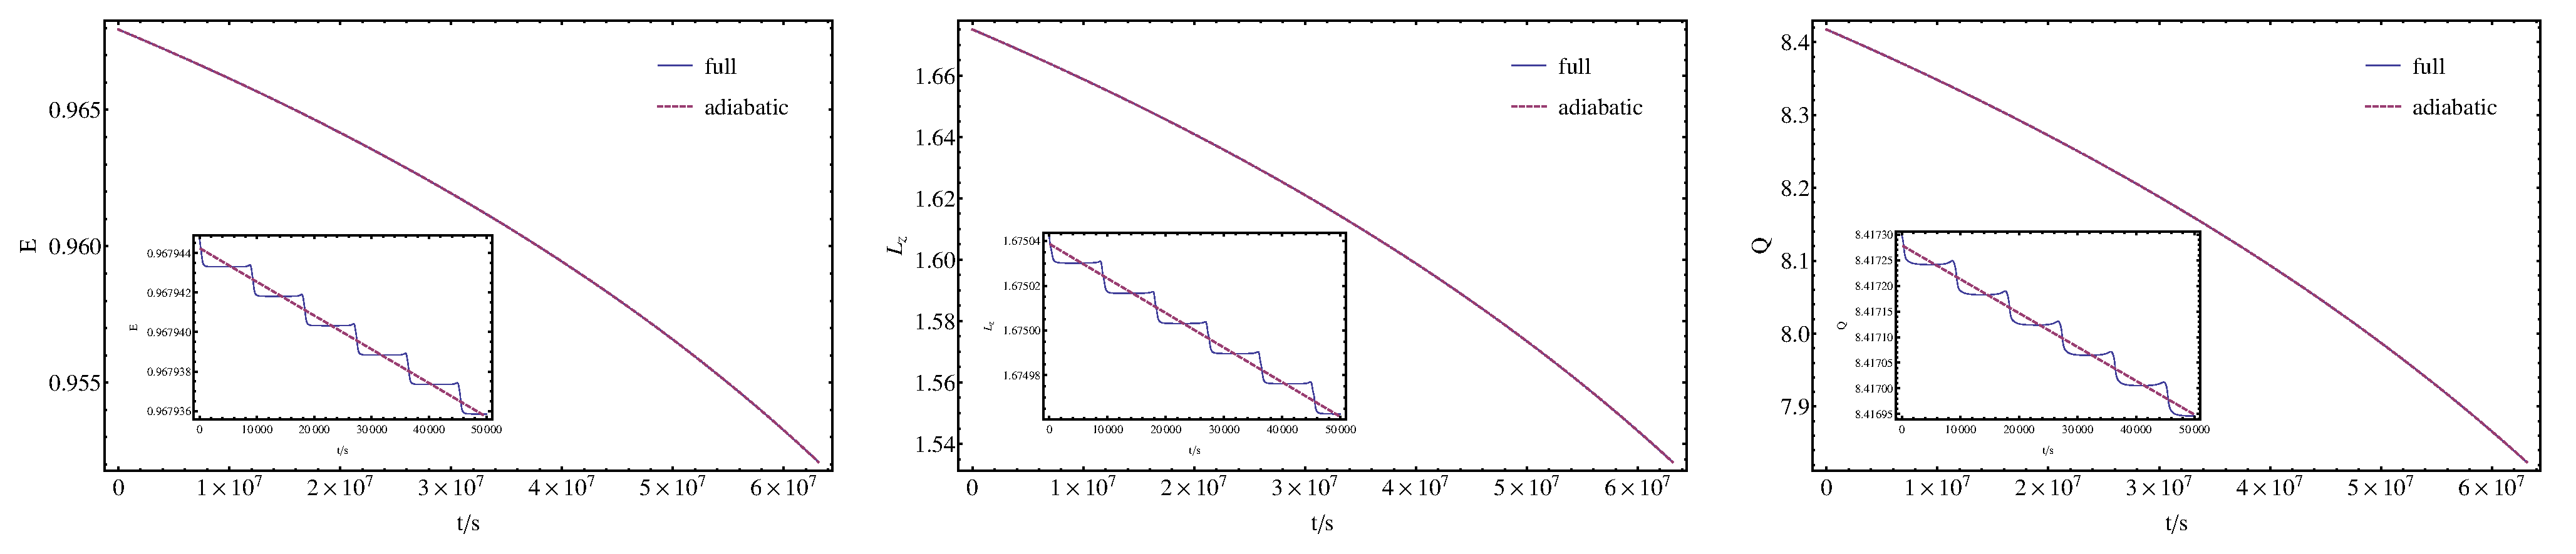
\includegraphics[width=\textwidth]{Fig_good_traj}
\caption{\label{fig:good-traj}The evolution of the orbital parameters $E$ (left), $L_z$ (center) and $Q$ (right) under the full (solid line) and adiabatic (dashed) models for an illustrative EMRI system that does not encounter any significant resonances. The inset plots show the behaviour on short timescales, where the fast orbital oscillations can be seen.}
\end{figure*}

\emph{Update this to reflect thesis.}

Once the trajectories have been computed using both methods of evolution, we can calculate the corresponding waveforms. The plus-polarised GW at the start and end of the evolution is shown in \figref{good-waveform}. The adiabatic waveform shows good agreement with the full waveform in both amplitude and phase. Calculating the SNR for each of the models, we find an overlap $\mathcal{O} = 0.984$, illustrating that adiabatic models can be used in place of the full evolution in cases where resonances are not encountered.

\begin{figure*}[htbp]
\centering
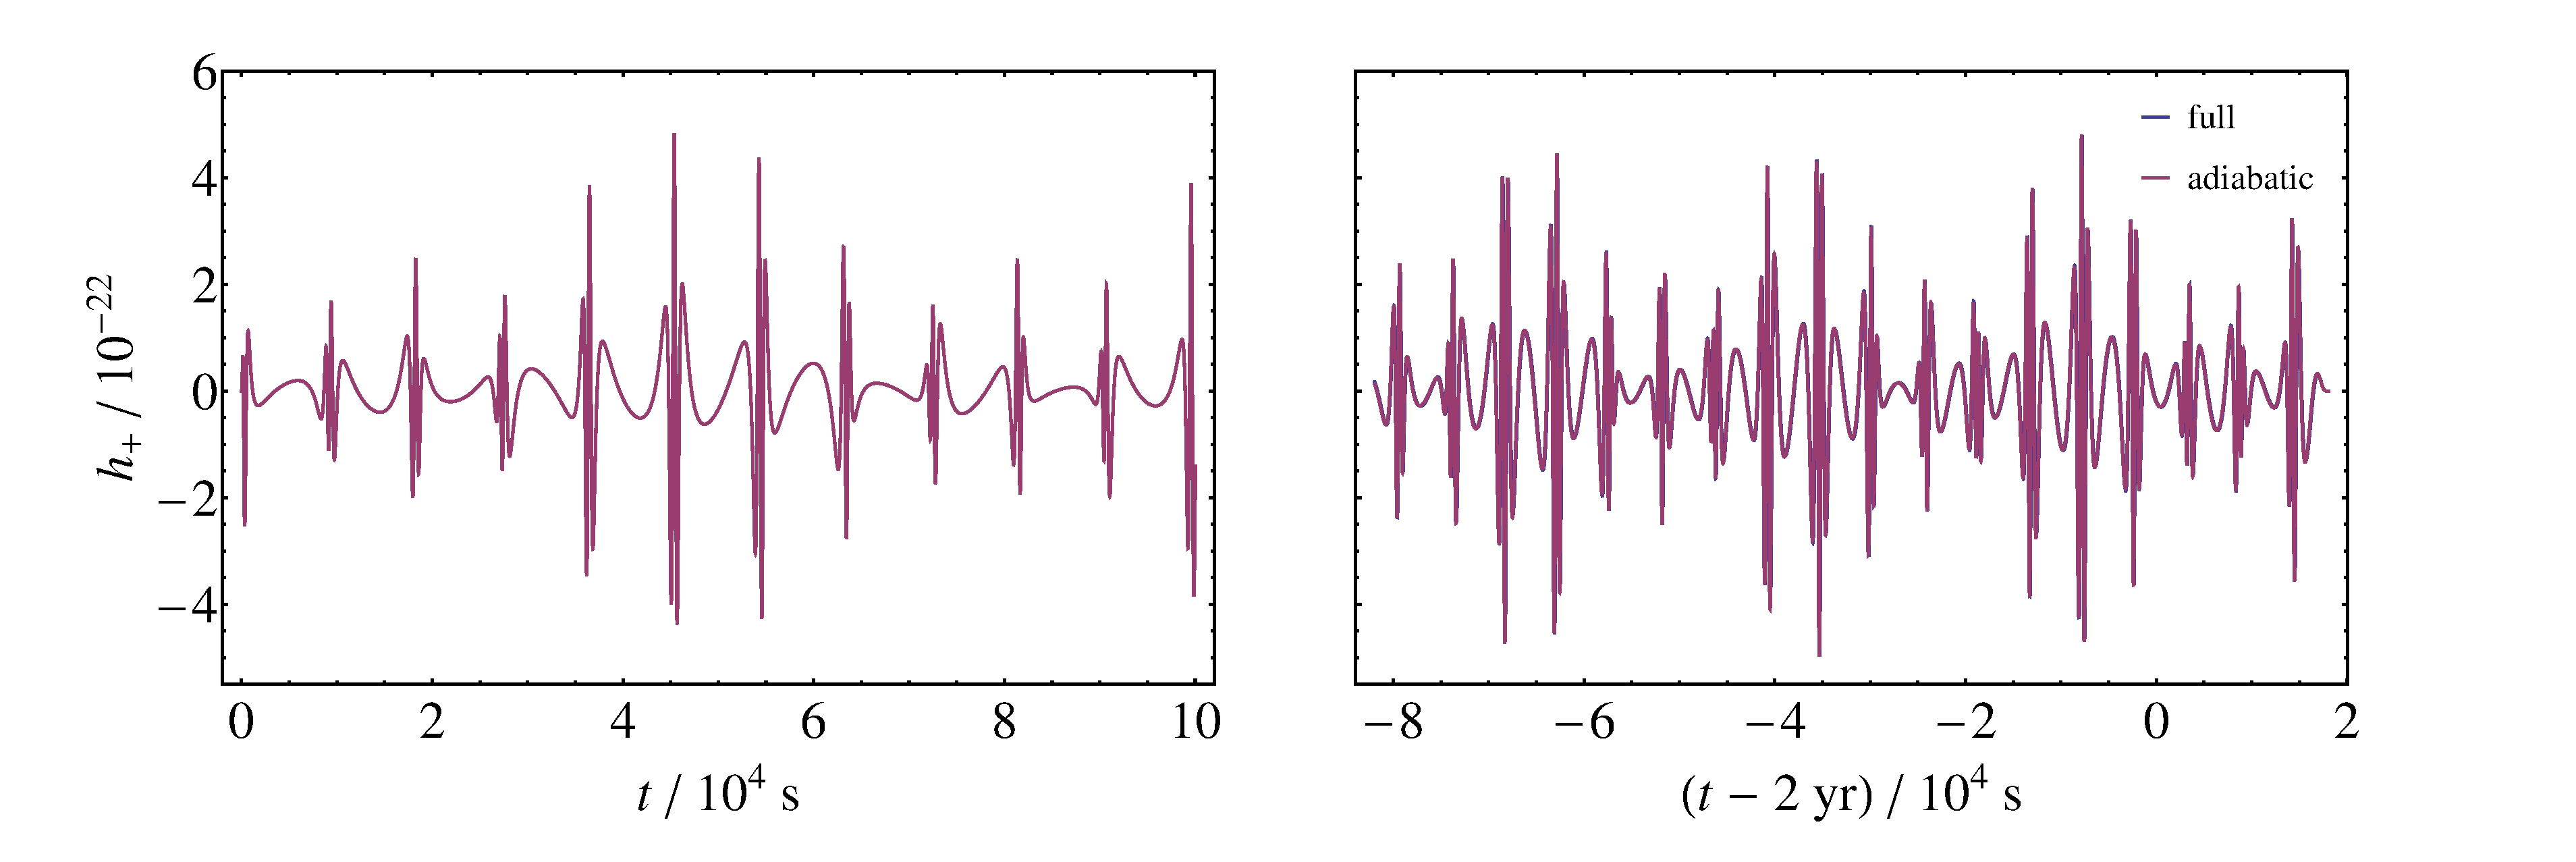
\includegraphics[width=0.92\textwidth]{Fig_good_waveform}
\caption{\label{fig:good-waveform}The plus-polarised waveform for an illustrative EMRI system with $p=7.5$, shown for two short segments at the start and end of a $2$ year evolution. The full and adiabatic models are both shown, but are indistinguishable by eye.}
\end{figure*}

\subsection{The effect of resonances: Dephasing}

The illustrative EMRI system of the previous section does not encounter a significant resonance and the adiabatic evolution provides a good match to the full evolution. We now study a system that does pass through a resonance during its $2$ year evolution. Specifically, we choose the initial conditions to be the same as before but with an initial semi-latus rectum $p=7.85$. This system passes through the 2:3 resonance, the effect of which is to cause a shift in the orbital parameters (and hence in the fundamental frequencies) that is not replicated by the adiabatic evolution, thus resulting in a rapid dephasing of the waveforms. Plotting the plus-polarised GWs at the start and end of the evolution, as before, demonstrates this dephasing, as shown in \figref{dephased-waveform}.

\begin{figure*}[htbp]
\centering
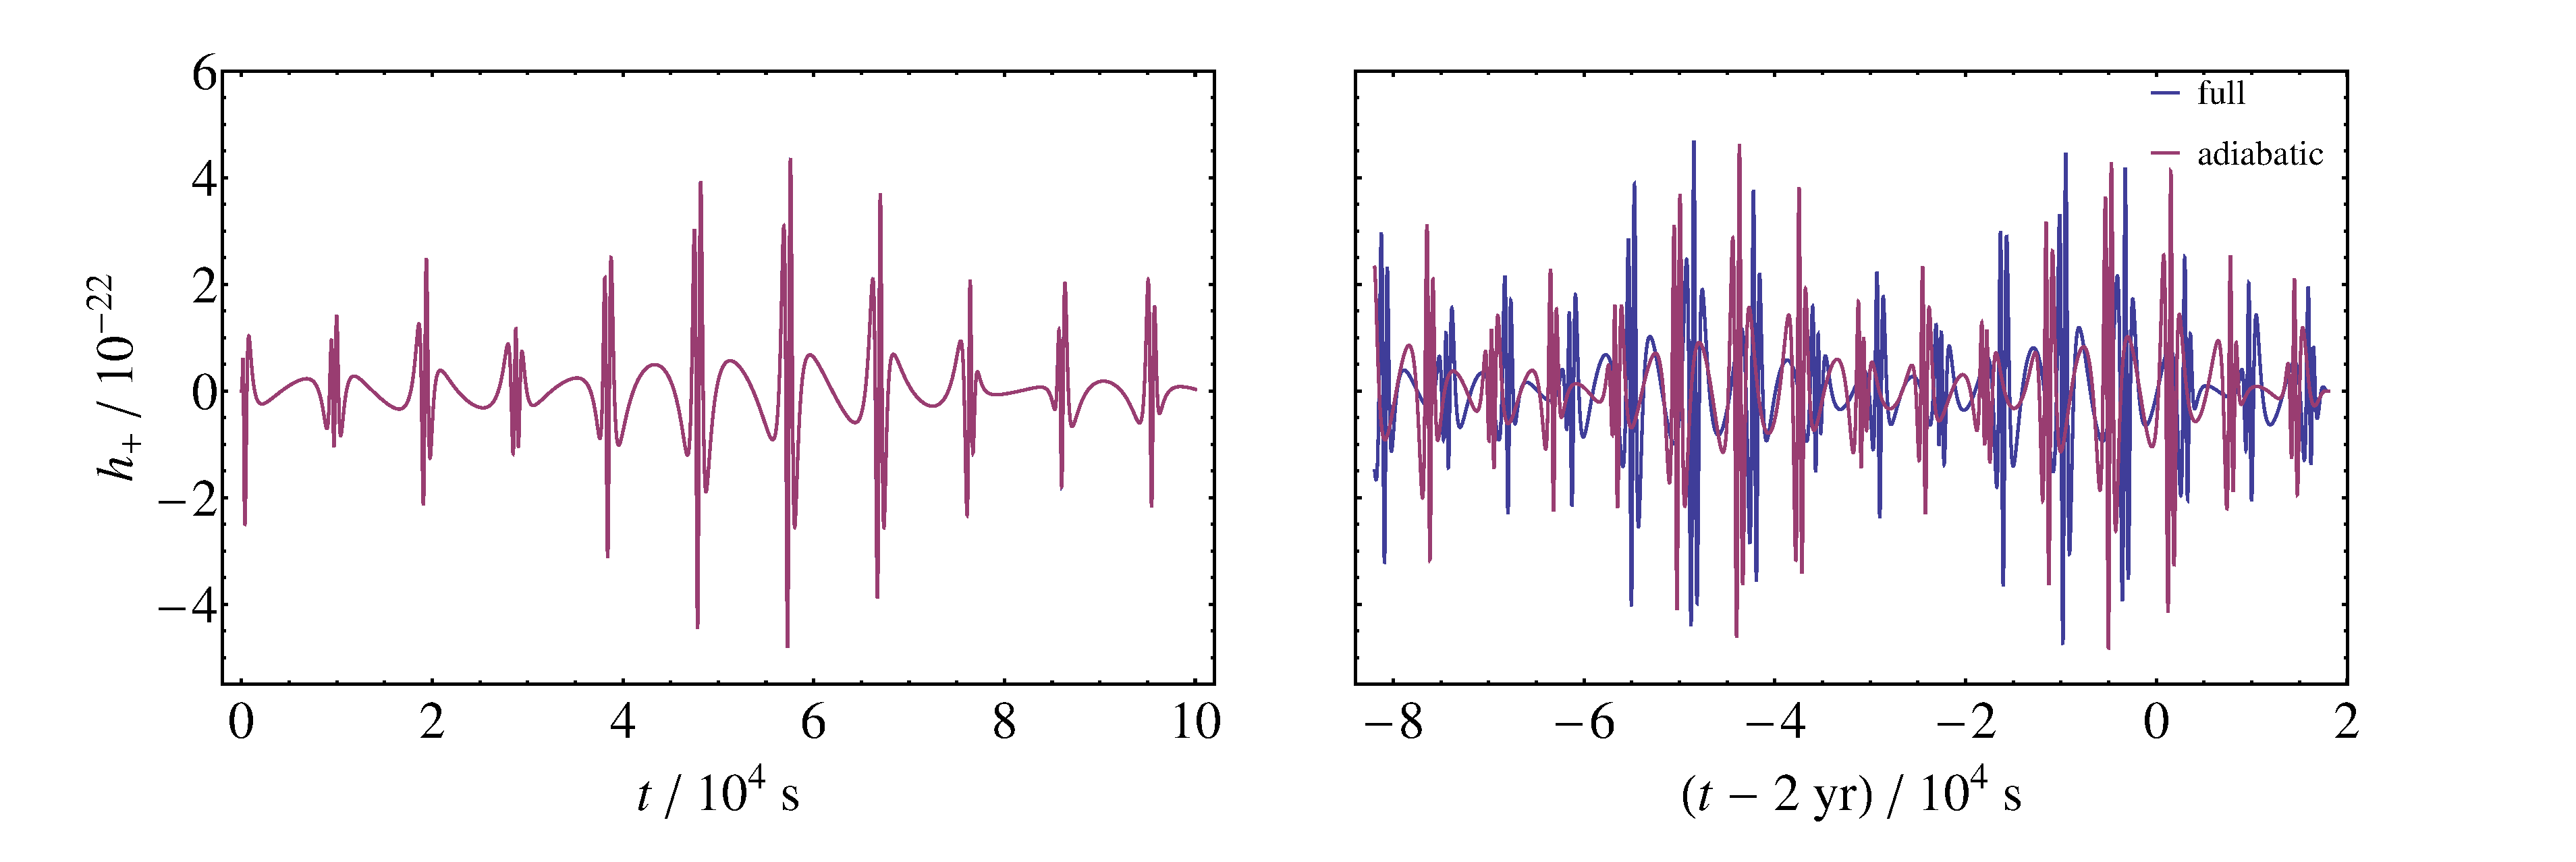
\includegraphics[width=0.92\textwidth]{Fig_dephased_waveform}
\caption{\label{fig:dephased-waveform}The plus-polarised waveform for an illustrative EMRI system with $p=7.85$, shown for two short segments at the start and end of a $2$ year evolution. The full and adiabatic models are both shown; there is a significant dephasing between them by the end of the evolution.}
\end{figure*}

To highlight the dephasing more quantitatively, we calculate the shortened overlap between the two models as a function of time $t$, defined as the overlap obtained by including only the part of the waveform within some $\Delta t$ of $t$. For our illustrative system, we choose $\Delta t$ such that we can calculate 25 non-overlapping values of this shortened overlap. Before the resonance occurs, the adiabatic model provides a good match to the full evolution but the overlap is reduced near to the resonance and never fully recovers afterwards. This is shown in \figref{overlap-dephasing}, which is centered on the time at which the full evolution crosses the 2:3 resonance.

\begin{figure}[htbp]
\centering
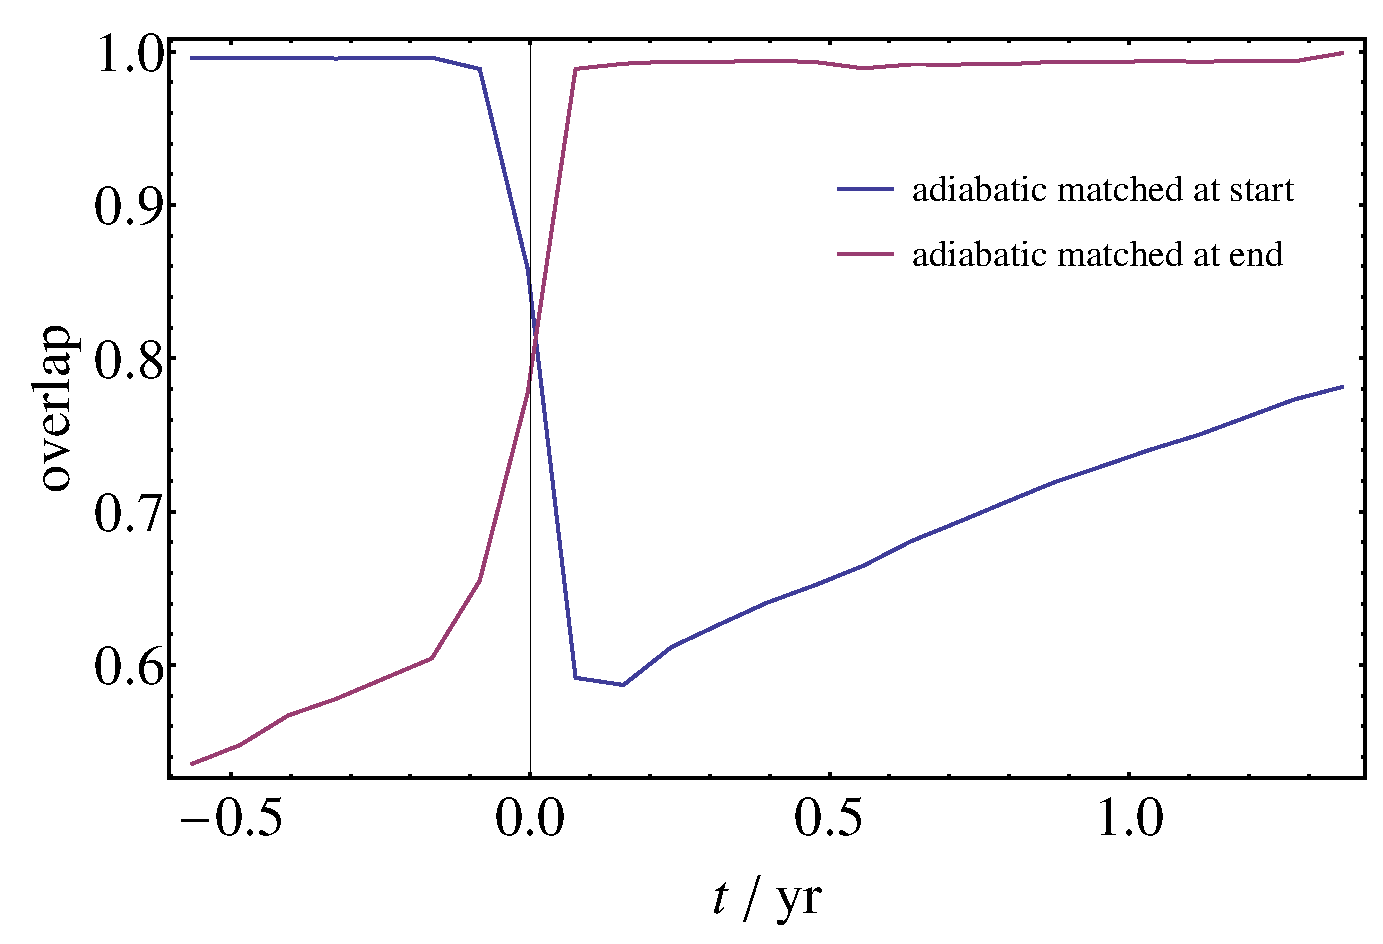
\includegraphics[width=0.46\textwidth]{Fig_overlap_vs_time}
\caption{\label{fig:overlap-dephasing}The overlap computed between the full evolution and an adiabatic evolution for an illustrative EMRI system with $p=7.85$, as a function of time, including only the parts of the waveforms within some $\Delta t$ of $t$, arbitrarily chosen to give 25 independent (non-overlapping) calculations. The time axis is centred on the value at which the full evolution crosses the 2:3 resonance.}
\end{figure}

Also shown is the shortened overlap computed between the full evolution and a different adiabatic evolution that is chosen to match the full evolution at the end of the integration. In this case, we see similar behaviour as before: the adiabatic waveform has a high overlap in the region where it is constructed to match the full evolution and the boundary of that region is set by the presence of an important resonance.

\subsection{The effect of resonances: Loss of SNR}
\label{sec:SNRloss}

\emph{Update this to reflect thesis.}

To be able to quantify the effect that the resonance has on an evolution, we turn to the SNR and the overlap between full and adiabatic models computed for the entire length of the observed inspiral. The dephasing means that an adiabatic evolution with the same initial conditions as a full evolution is likely to have a low overlap if a significant resonance is encountered. However, this does not necessarily mean that all adiabatic evolutions have low overlaps; we need to search for optimal adiabatic parameters, such that the overlap is maximal.

The extremely large parameter space of adiabatic waveforms renders a brute-force approach computationally impossible; it is therefore necessary to restrict the search in some way. For this preliminary investigation into the importance of resonances, we do this by focussing on a small subset of parameters that we suspect will produce a large overlap. We make the assumption that a good adiabatic model will \emph{exactly} match the full model at some time $t_{\mathrm{match}}$. This reduces the search to a one parameter family of waveforms that can easily be computed concurrently with the full evolution.

The most restrictive aspect of this approach is that all extrinsic parameters and any intrinsic ones that remain constant throughout the evolution, such as the masses of the BHs and the central BH spin, do not get explored by our family of adiabatic models. It is possible that small deviations from these true parameters give rise to better matching adiabatic models, to partially correct for the (lack of) resonance effects. Indeed, systematic biases are expected when the model waveforms do not accurately reflect the data~\cite{Cutler2007}.

The problem of searching over adiabatic templates now reduces to the task of choosing appropriate values of $t_{\mathrm{match}}$. Anticipating that resonances shall play a key role in determining the degree of waveform overlap, we choose matching times situated at $5\tau_\mathrm{res}$ after each resonance of interest, namely the low-order 2:3, 1:2, 2:5 and 1:3. These matching times lie in a portion of the evolution that is not affected by a resonance and so should result in a large overlap for that region of the inspiral. We also include templates that match at the start of the evolution, so that we have a model that should match the portion of the evolution before the first resonance, and at the end of the evolution, as this is often where most SNR is accumulated. In addition, we include models that match exactly on each of the resonances as these may achieve partial matching both before and after the resonance and hence perform well.

We have tried a more rigid system of choosing the values of $t_{\mathrm{match}}$, producing an adiabatic evolution regularly at fixed intervals, but these generally perform no better than our adaptive match points and require many more adiabatic evolutions to be calculated.

In our experience, we found that these choices were not sufficient to produce a good family of adiabatic waveforms. In particular, if an adiabatic model happened to match the full model close to a turning point in the fast orbital evolution, then it eventually diverged from the full model and the resulting waveform provided a poor match. We therefore adjust the values of $t_{\mathrm{match}}$ so that they correspond to times in the inspiral when the time-derivative of a particular orbital parameter (we choose the semi-latus rectum $p$) is maximally different from the adiabatic time-derivative of that orbital parameter. This ensures that the adiabatic model intersects with the full model close to the centre of the envelope created by the fast oscillations, as demonstrated by the inset plots in \figref{good-traj}, and as a result gives much higher overlaps in general.

For the illustrative EMRI system detailed in the previous section, we have computed the family of adiabatic models set by $t_{\mathrm{match}}$ and the resulting trajectories are consistent for the length of the evolution. As they cannot be easily distinguished by eye, we plot the difference (in $E$, $L_z$ and $Q$) between the models and the adiabatic evolution that matches at the start, shown in \figref{res-diff-traj}. The jumps in the orbital parameters due to the 2:3 resonance can be clearly seen, as can the fast orbital oscillations present in the full evolution but absent in the adiabatics.

\begin{figure*}[htbp]
\centering
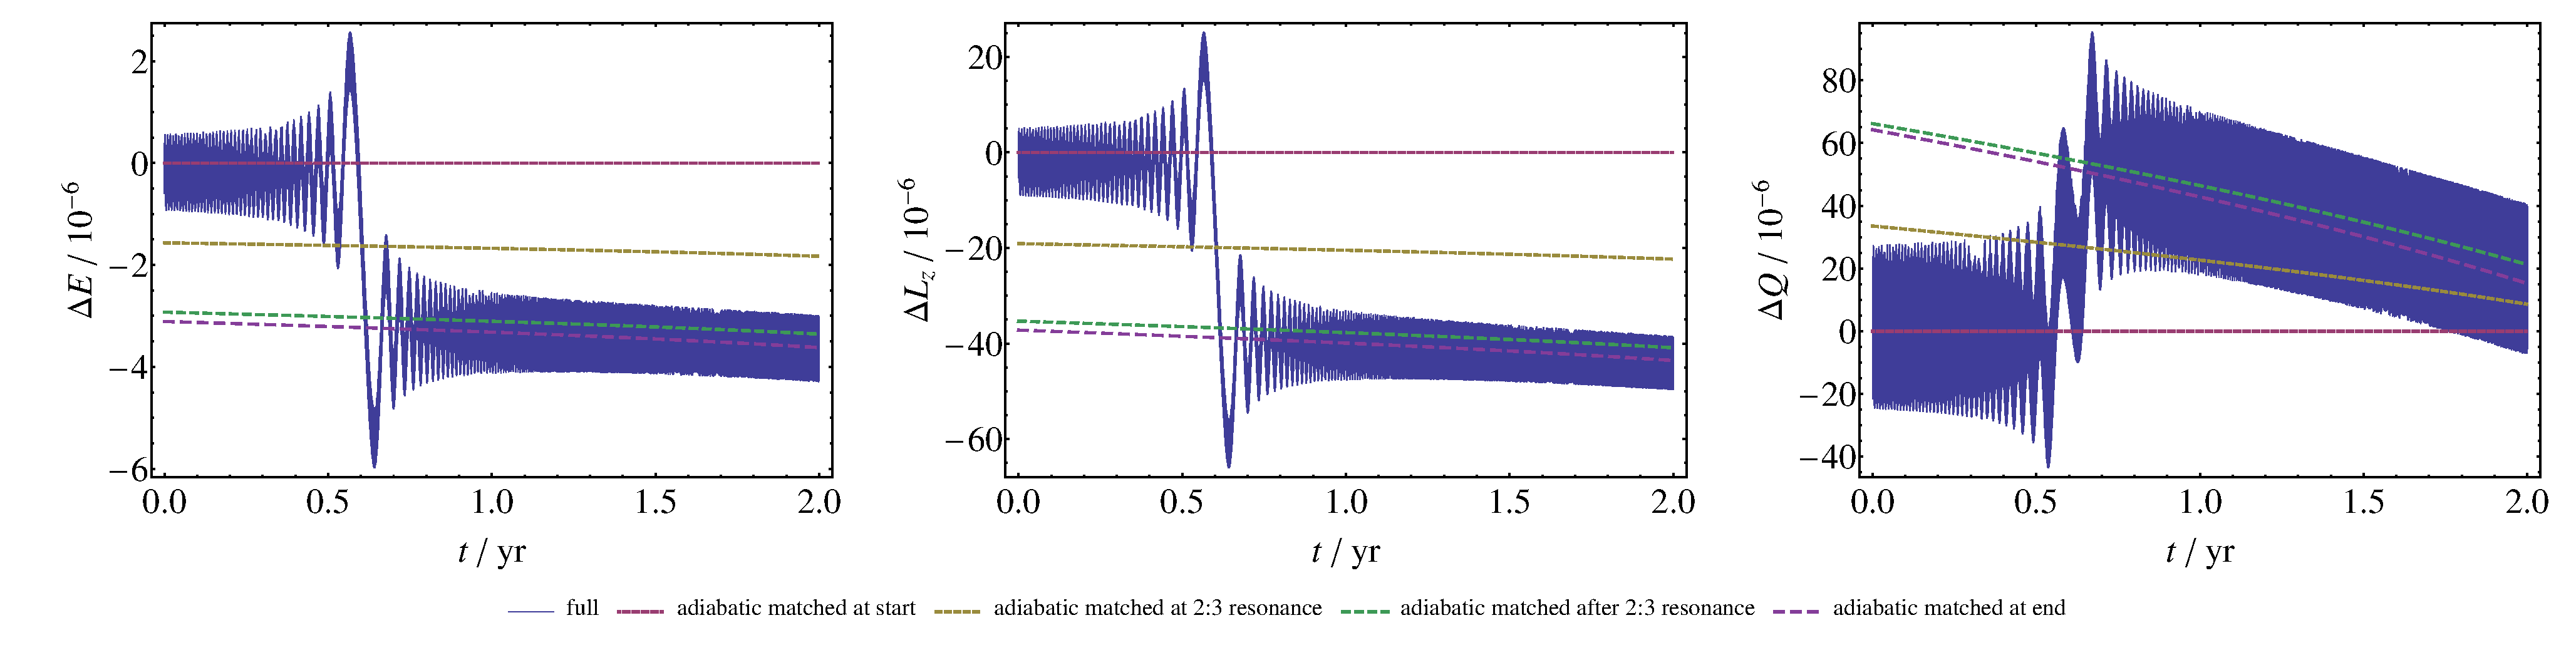
\includegraphics[width=\textwidth]{Fig_res_diff_traj}
\caption{\label{fig:res-diff-traj}The differences in orbital parameters $E$ (left), $L_z$ (center) and $Q$ (right) between each evolution scheme and the adiabatic model that matches at the start. The solid line shows the full evolution and the dashed lines show the different adiabatic evolutions, which match the full evolution at different times throughout the inspiral (numbers in parentheses give the overlap with the full evolution): at the start (0.202), at the 2:3 resonance (0.458), after the 2:3 resonance (0.259) and at the end (0.677).}
\end{figure*}

None of the adiabatic models presented here give a particularly high overlap with the full evolution, because of the effects of the resonance. The best-performing adiabatic model was that which matched at the end, giving $\mathcal{O} = 0.677$, while the model that matches at the start gives only $\mathcal{O} = 0.202$. These values can be explained qualitatively by the relative lengths of the adiabatic-like regions on either side of the resonance in the full evolution. 

\subsection{The effect of resonances: Jump sizes}

\emph{Update this to reflect thesis.}

As demonstrated in \figref{res-diff-traj} and computed analytically in \apref{res-asymptotic}, the full evolution undergoes a rapid change in the orbital parameters with respect to the adiabatic evolutions. To extract the magnitude of this jump from the trajectory data, we first must account for the fast orbital oscillations as well as ensuring that we include the full effect of the resonance, while minimising any changes resulting from other sources.

To achieve this, we isolate spans of data away from the resonance; specifically, looking at data that lies within five and ten resonance timescales away. For both the pre- and post-resonance datasets, we compute $\Delta \mathcal{I} \equiv \mathcal{I}_{\mathrm{full}} - \mathcal{I}_\mathrm{ad}[t_{\mathrm{match}} = t_\mathrm{res}]$ for each of the orbital parameters. We then identify the most horizontal straight lines that bound the data, which give an approximation to the behaviour of the fast orbital oscillations. The resulting data and bounding lines are shown for our illustrative system in \figref{res-jump-calc}.

\begin{figure}[htbp]
\centering
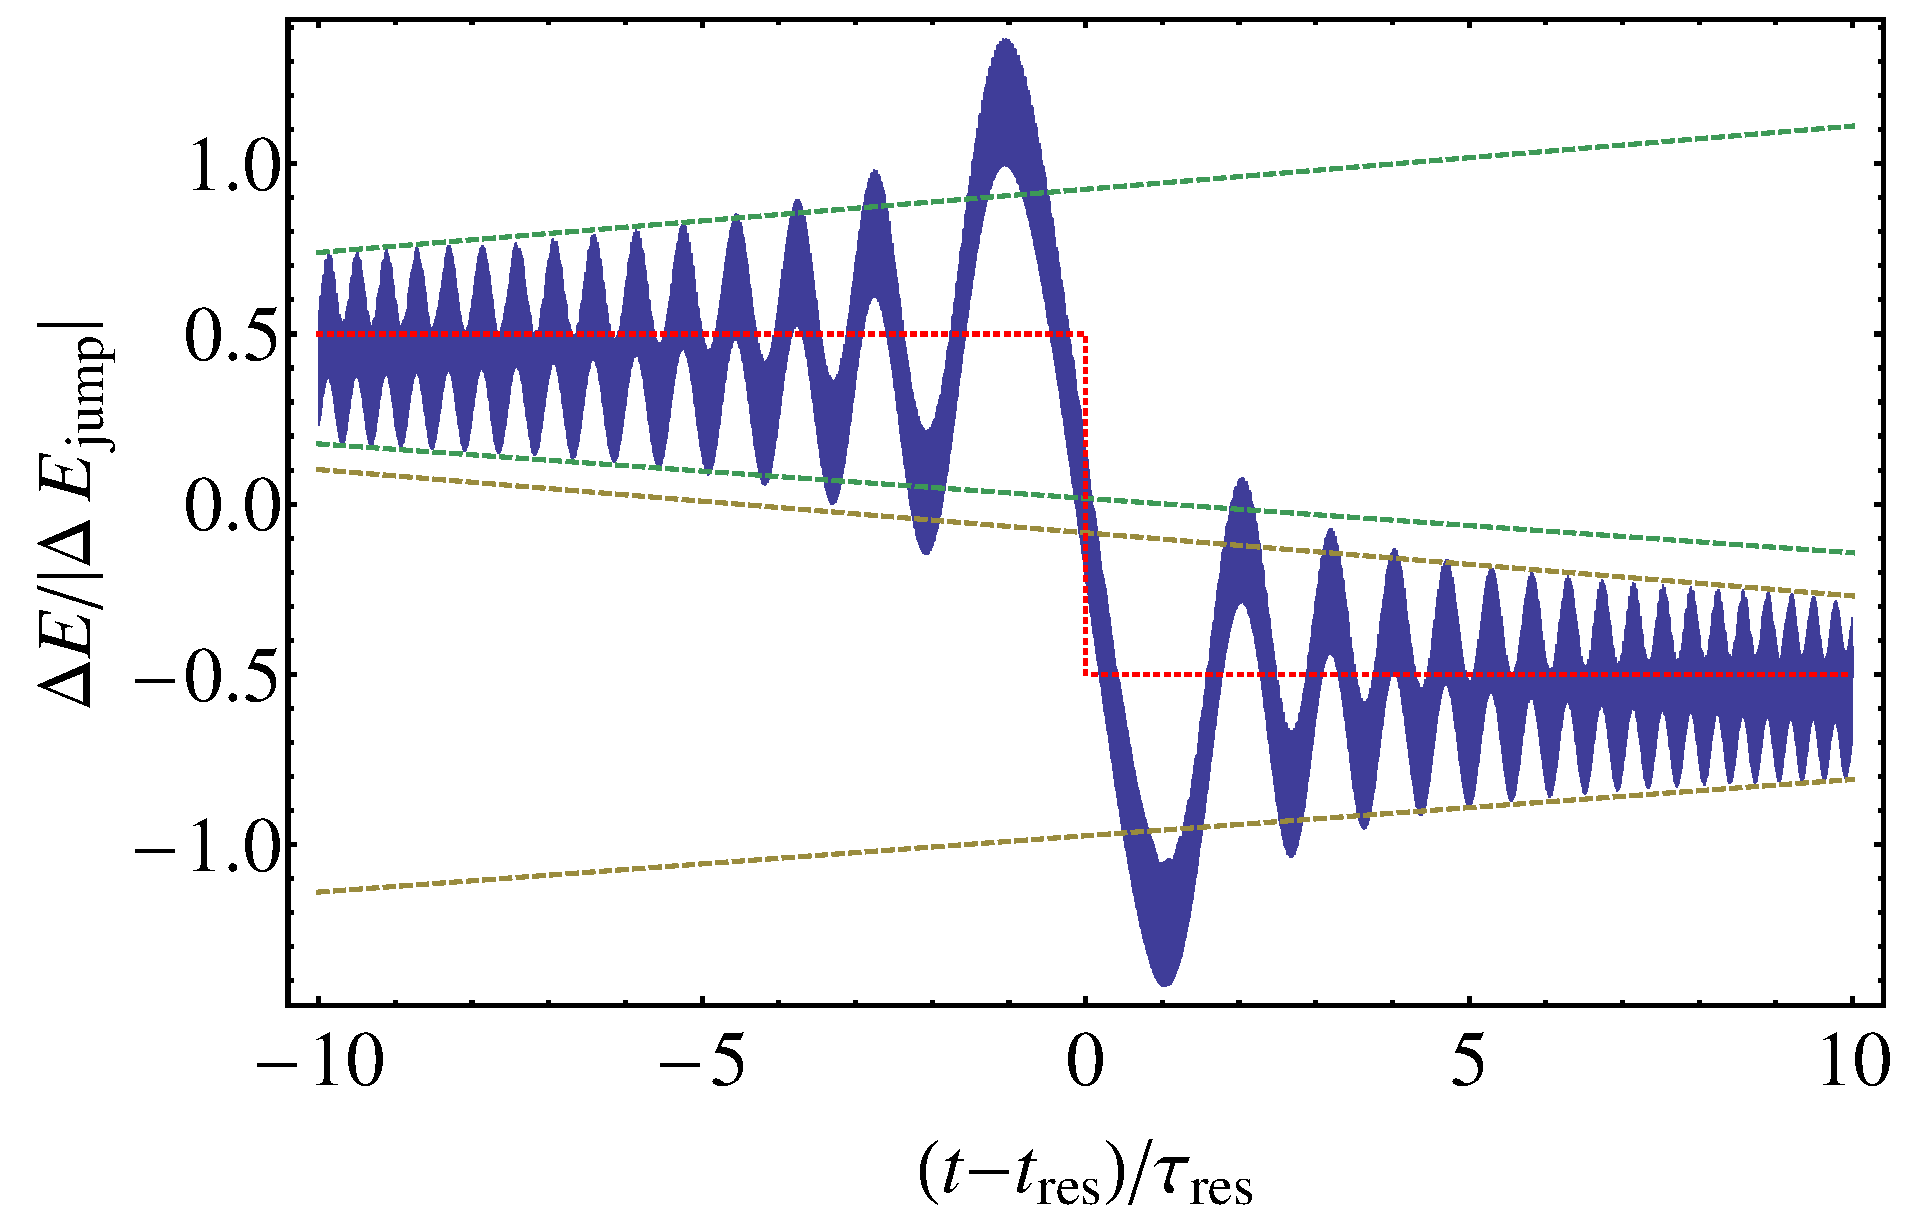
\includegraphics[width=0.46\textwidth]{Fig_res_jump_calc}
\caption{\label{fig:res-jump-calc}The difference in energy between the instantaneous model and adiabatic model that matches at the 2:3 resonance, scaled by the magnitude of the 2:3 resonance jump. The dashed green (yellow) lines show the bounding fits to the data before (after) the resonance, used to numerically estimate the size of the jump. The dotted red line indicates the computed size of the jump. The time axis is centred on the 2:3 resonance and is scaled by the appropriate resonance timescale.}
\end{figure}

To estimate the size of the jump $\Delta \mathcal{I}_{\mathrm{jump}}$, we extrapolate the bounding lines to the resonance time and calculate the difference between the pre- and post-resonance values, quoting the final result as the average of that obtained using the upper and lower limits. This allows us to take into account any linear drift in $\Delta \mathcal{I}$ that can occur over the resonance timescale due to the inaccuracy of the adiabatic approximation. In addition, by using information from both the upper and lower limits, we can veto jump calculations that appear erroneous: if one jump is positive and the other negative, then we ignore that resonance; this often occurs very near to plunge, where the adiabatic approximation breaks down. For typical systems, this numerically computed jump appears to well describe the resonance, as shown by the red dotted line in \figref{res-jump-calc}.

The absolute size of the resonance jump is often not particularly useful, especially when comparing different systems. Instead, we can express the resonance jump as a fraction of the adiabatic change expected across the resonance. For the orbital parameter $\mathcal{I}$,
\begin{equation}
\label{eq:res-jump-ratio}
\frac{\Delta \mathcal{I}_\mathrm{jump}}{\mathcal{I}_\mathrm{ad}(t>t_\mathrm{res})-\mathcal{I}_\mathrm{ad}(t<t_\mathrm{res})} = \frac{\Delta \mathcal{I}_\mathrm{jump}}{\dot{\mathcal{I}}_\mathrm{ad}(t_\mathrm{res})\tau_\mathrm{res}}.
\end{equation}

The resonance jump depends sensitively on the relative phase of radial and poloidal motions. It is therefore instructive to study the resonance problem using an ensemble of systems differing only in the initial value of the radial phase $\psi$, which we do for our illustrative system parameters. Choosing random values for $\psi$ corresponds to random values of the orbital phase on resonance $\widehat{\kappa}_0$, which should map out the full range of resonance jumps for these particular orbital shape parameters, according to \eqnref{delta-I-a}.

Given our computed resonance jumps for all of the orbital parameters, we extract a single phase parameter $q$ for each system that specifies the magnitude of each jump. We expect such a phase parameter to be linearly offset from $\widehat{\kappa}_0$. The resonance jumps are sinusoidal with respect to $q$, as shown by the fits in \figref{resjump-vs-q}, lending support to \eqnref{delta-I-a} and giving us confidence in our numerical jump calculations. We can also compute the jumps in the fundamental frequencies for each system (shown as dashed lines in \figref{resjump-vs-q}).

\begin{figure}[htbp]
\centering
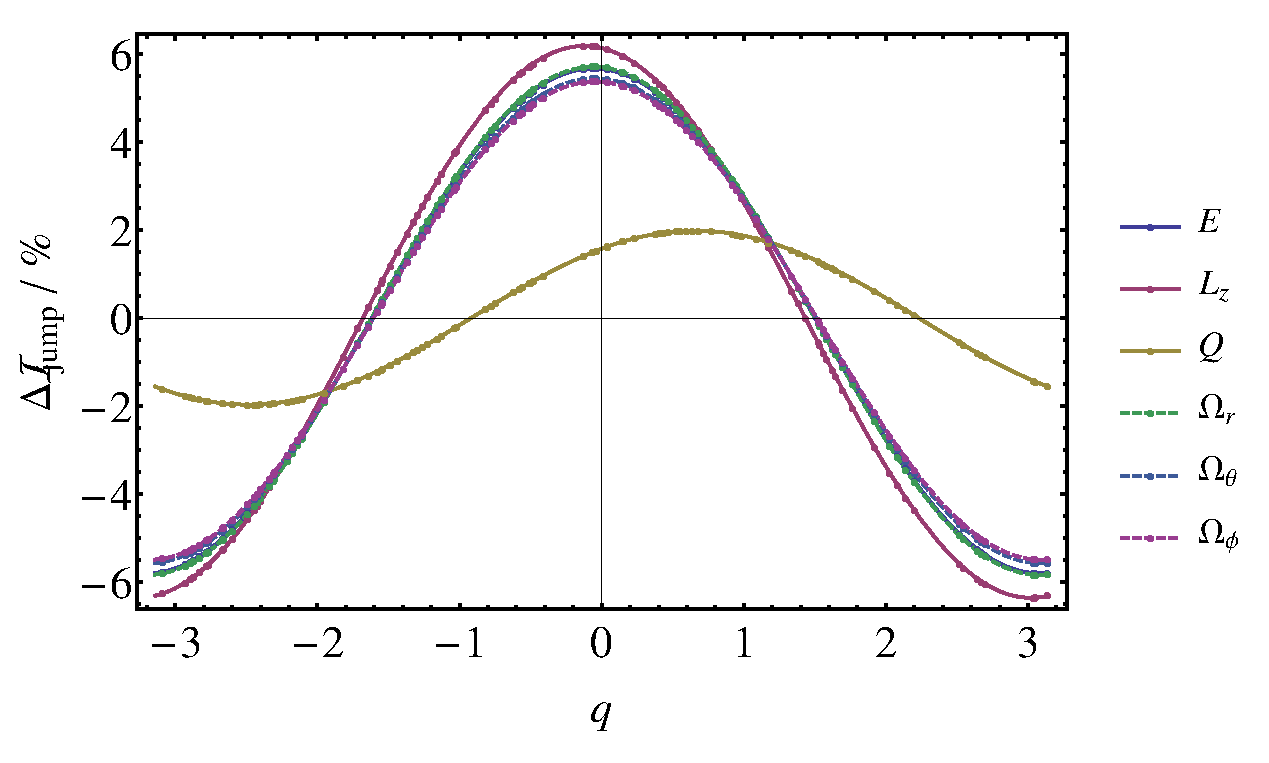
\includegraphics[width=0.46\textwidth]{Fig_jump_vs_q}
\caption{\label{fig:resjump-vs-q}The magnitude of the resonance jump for our illustrative system as a function of the extracted phase parameter $q$. The jump is expressed as a percentage of the adiabatic change in each parameter, given by \eqnref{res-jump-ratio}. The individual jumps as well as a sinusoidal fit are plotted for the three orbital shape parameters (solid lines) and the three orbital frequencies (dotted).}
\end{figure}

For each system, we compute the overlap between the full evolution and the family of adiabatics given by our set of match times $t_\mathrm{match}$ described in the previous section. The largest overlap in each case is plotted in \figref{overlap-vs-resjump-ill}, as a function of the percentage resonance jumps in the orbital parameters. We observe no strong trend with the size of the jump, although systems with small jumps in $E$ (less than $1\%$) have higher than average overlaps. These systems also have small jumps in the fundamental frequencies and so the adiabatic waveform dephases more slowly from the full waveform, leading to a larger overlap.

\begin{figure*}[htbp]
\centering
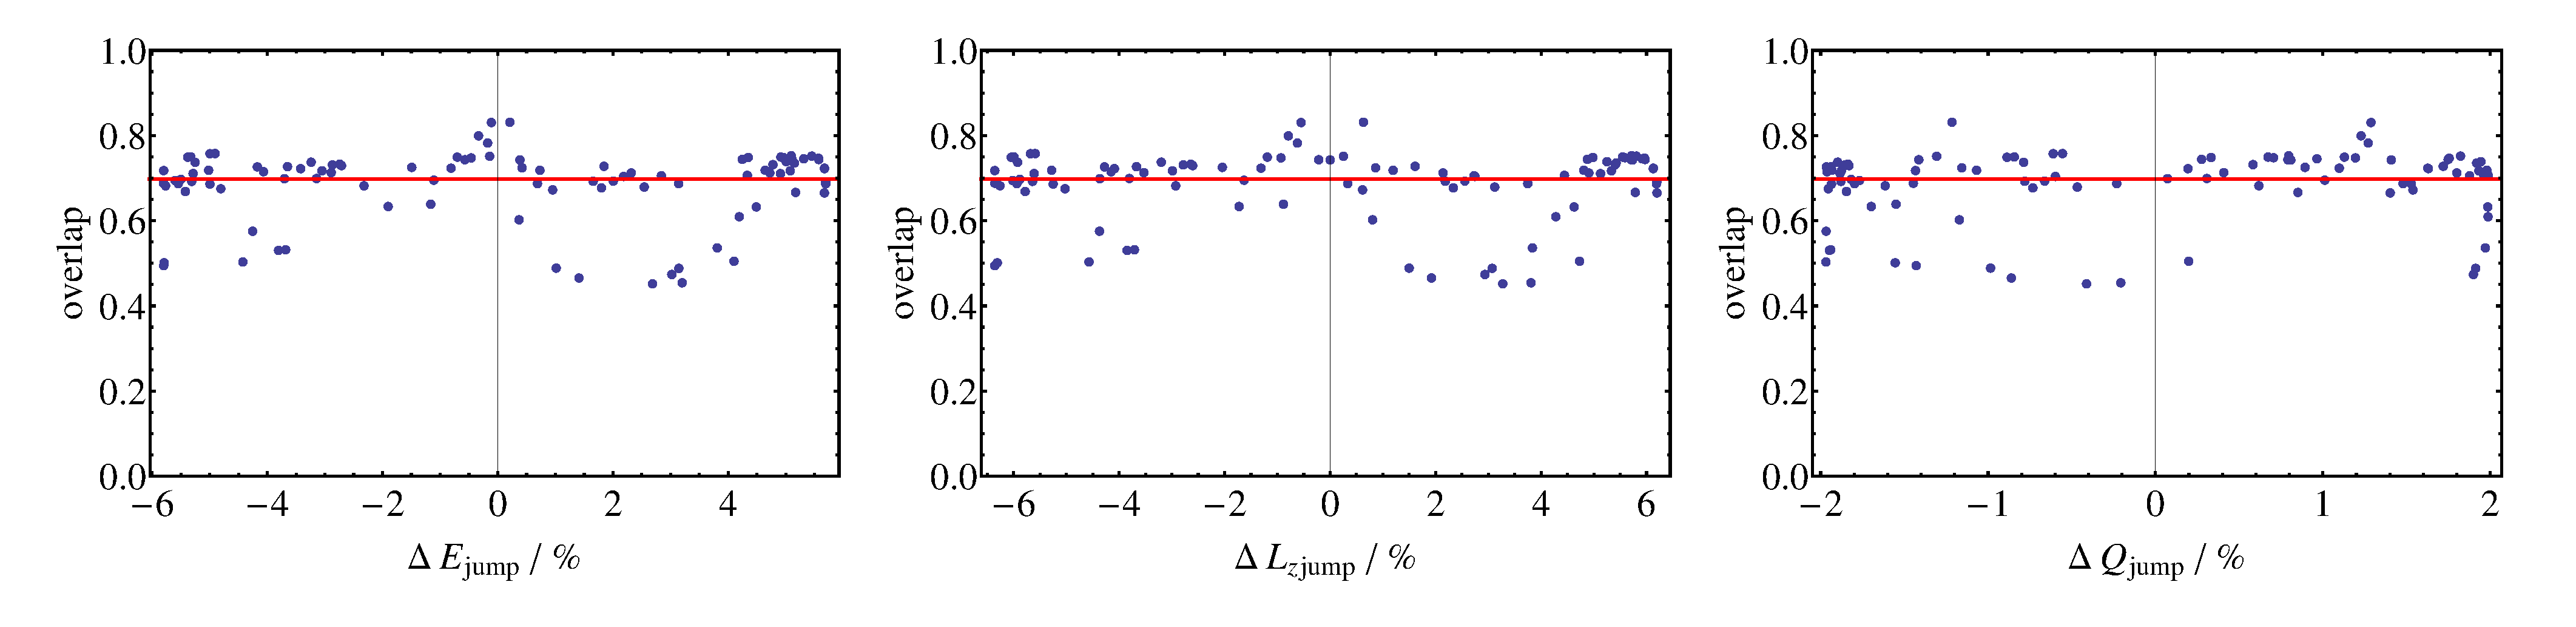
\includegraphics[width=\textwidth]{Fig_overlap_vs_resjump_ill}
\caption{\label{fig:overlap-vs-resjump-ill}The overlap \eqnref{overlap} between the full and adiabatic evolutions, maximised over the family of generated adiabatics, as a function of the resonance jumps in $E$ (left), $L_z$ (middle), and $Q$ (right). Each dot represents a system with our illustrative parameters and a random choice of the initial radial phase. The red line indicates the expected overlap assuming that the waveforms match exactly post-resonance, but have zero overlap pre-resonance.}
\end{figure*}

The best performing adiabatic for the majority of our systems matched at the end of the inspiral. We can interpret the low overlaps by assuming that these adiabatic waveforms recover the entire SNR in the region post-resonance, but none pre-resonance. As a result, we would expect the overlap to roughly equal the fraction of time spent post-resonance, which in this case is $0.7$, demonstrated by the red line in \figref{overlap-vs-resjump-ill}. There is not an exact equivalence because of the frequency-dependent noise of eLISA; cycles near the end of the inspiral accumulate proportionally more SNR at a frequency closer to the base of the eLISA noise curve.

A small fraction of systems have a much lower overlap than expected, at around $0.5$. This is due to a sub-optimal choice of the matching times; making small adjustments to $t_\mathrm{match}$ can lead to higher overlaps around $0.7$, but the exact adjustments required are difficult to predict in advance.


\subsection{Sample EMRI population}

\emph{COMPLETELY REWRITE}

\emph{Basically summarise the GOAT population. Maybe include event rate estimates in appendix??}

Strong resonances can severely limit our ability to recover SNR from waveforms using adiabatic templates; they partition the inspiral, splitting up the total SNR into different adiabatic modes, which may be individually undetectable. To assess the impact of this on future GW missions, we need to create a sample population of detectable EMRIs.

We first identify 14 parameter distributions that describe an astrophysically typical EMRI\footnote{The actual distribution in parameter space of observable EMRI systems is unknown, but we can make reasonable estimates.}. We choose the mass of the compact object $\mu = 10 M_\odot$, corresponding to a typical mass for stellar BHs. We take the central object to be a typical supermassive BH at the centre of a galaxy, with mass $M$ uniformly distributed in log-space between $10^5 M_\odot$ and $10^7 M_\odot$, and dimensionless spin $a_\ast$ uniformly between its limiting values, $0$ and $1$. The direction of the spin of the central BH, the direction of the angular momentum of the orbit and the direction of the source on the sky are all chosen uniformly on the sphere. The angles specifying the location of pericenter and the compact object around the orbit are distributed uniformly between $0$ and $2\pi$.

We assume a standard cosmology with $\Omega_\Lambda = 0.7$, $\Omega_m = 0.3$ and $H_0 = 70\,\mathrm{km s^{-1}\, Mpc^{-1}}$, and sample the redshift of the source uniformly from comoving volume, up to a maximum of $z_\mathrm{max} = 0.7$. We don't expect the exact details of the cosmology to significantly alter our results and our choice of $z_\mathrm{max}$ is justified \textit{post hoc}.

The astrophysics in dense stellar clusters at the center of galaxies leading to EMRI production is highly uncertain. The currently favoured formation mechanism scatters compact objects onto highly eccentric orbits, which lose a burst of energy to GW emission with each periapse passage. This tends to circularise the orbit, as the compact object spirals inwards. Hopman and Alexander \cite{Hopman2005} model this scattering and give an eccentricity distribution for compact objects spiralling into a $3 \times 10^6 M_\odot$ Schwarzschild BH at the point when the orbital period enters the LISA band at $10^4\,\mathrm{s}$. The overall results of their work are still valid for spinning BHs and so assuming that this distribution holds for other BH masses, we can sample the orbit eccentricity and calculate the semi-latus rectum from the orbital period.

These EMRIs are astrophysically motivated, but may not be detectable by eLISA. To assess this, we evolve the systems forward in time using the analytic kludge method of Barack and Cutler \cite{Barack2004} until they reach the last stable orbit. We then calculate the Peters-Matthews waveform \cite{Peters1963} for a time $t_\mathrm{insp}$ at the end of the inspiral, where $t_\mathrm{insp}$ is chosen uniformly between $0.5$ years and $2$ years. We focus on the late stages of inspiral as these are most likely to be detected by eLISA. Given the waveform, we can estimate the expected SNR by approximating the overlap with a time-domain integral
\begin{equation}
\overlap{s}{h} \approx 4 \intd{0}{t_\mathrm{insp}}{\frac{s(t)h(t)}{S_n(f(t))}}{t},
\end{equation}
where $f(t)$ is some characteristic frequency of the orbit at time $t$. We find that taking $f$ to be twice the (radial) orbital frequency gives a good approximation to the SNR.

To obtain our final distribution of detectable EMRIs, shown as dark blue in \figref{EMRIpar-dists}, we quote the parameter values $t_\mathrm{insp}$ before plunge. Only systems with $\rho > 10$ are treated as detectable. Also shown in the figure, in light pink, are the systems with an estimated SNR below 10, to illustrate which systems tend to have lower SNRs. The acceptance rate for generating a detectable EMRI from the entire distribution is $32\%$.

We note that prograde orbits (those with $\cos\iota > 0$) and systems with higher BH spins tend to be favoured; this is likely due to the fact that such systems can inspiral much closer before finally plunging, and so experience the strongest gravitational fields. This effect is amplified by the fact that the majority of the SNR is recovered from the final part of the inspiral, which also explains why larger values of $t_\mathrm{insp}$ are only marginally preferred over smaller values.

Systems at higher redshifts start to become undetectable as the amplitude of the signal scales inversely proportional to the luminosity distance to the source. At $z=0.7$, the fraction of detectable systems drops to $5\%$; this is chosen as the upper limit in the redshift distribution to minimise unneccessary computations. We quote the masses in the system as redshifted masses, which accounts for the frequency shift due to the expansion of the Universe.

The circularising effect of GW emission can be observed in the eccentricity distribution: even though the input systems from Hopman and Alexander have high eccentricites, with a peak in the distribution at $e\sim0.7$, the final distribution contains only low eccentricity systems, peaked at $e\sim0.05$ with a maximum at $e=0.31$.

\begin{figure*}[htbp]
\centering
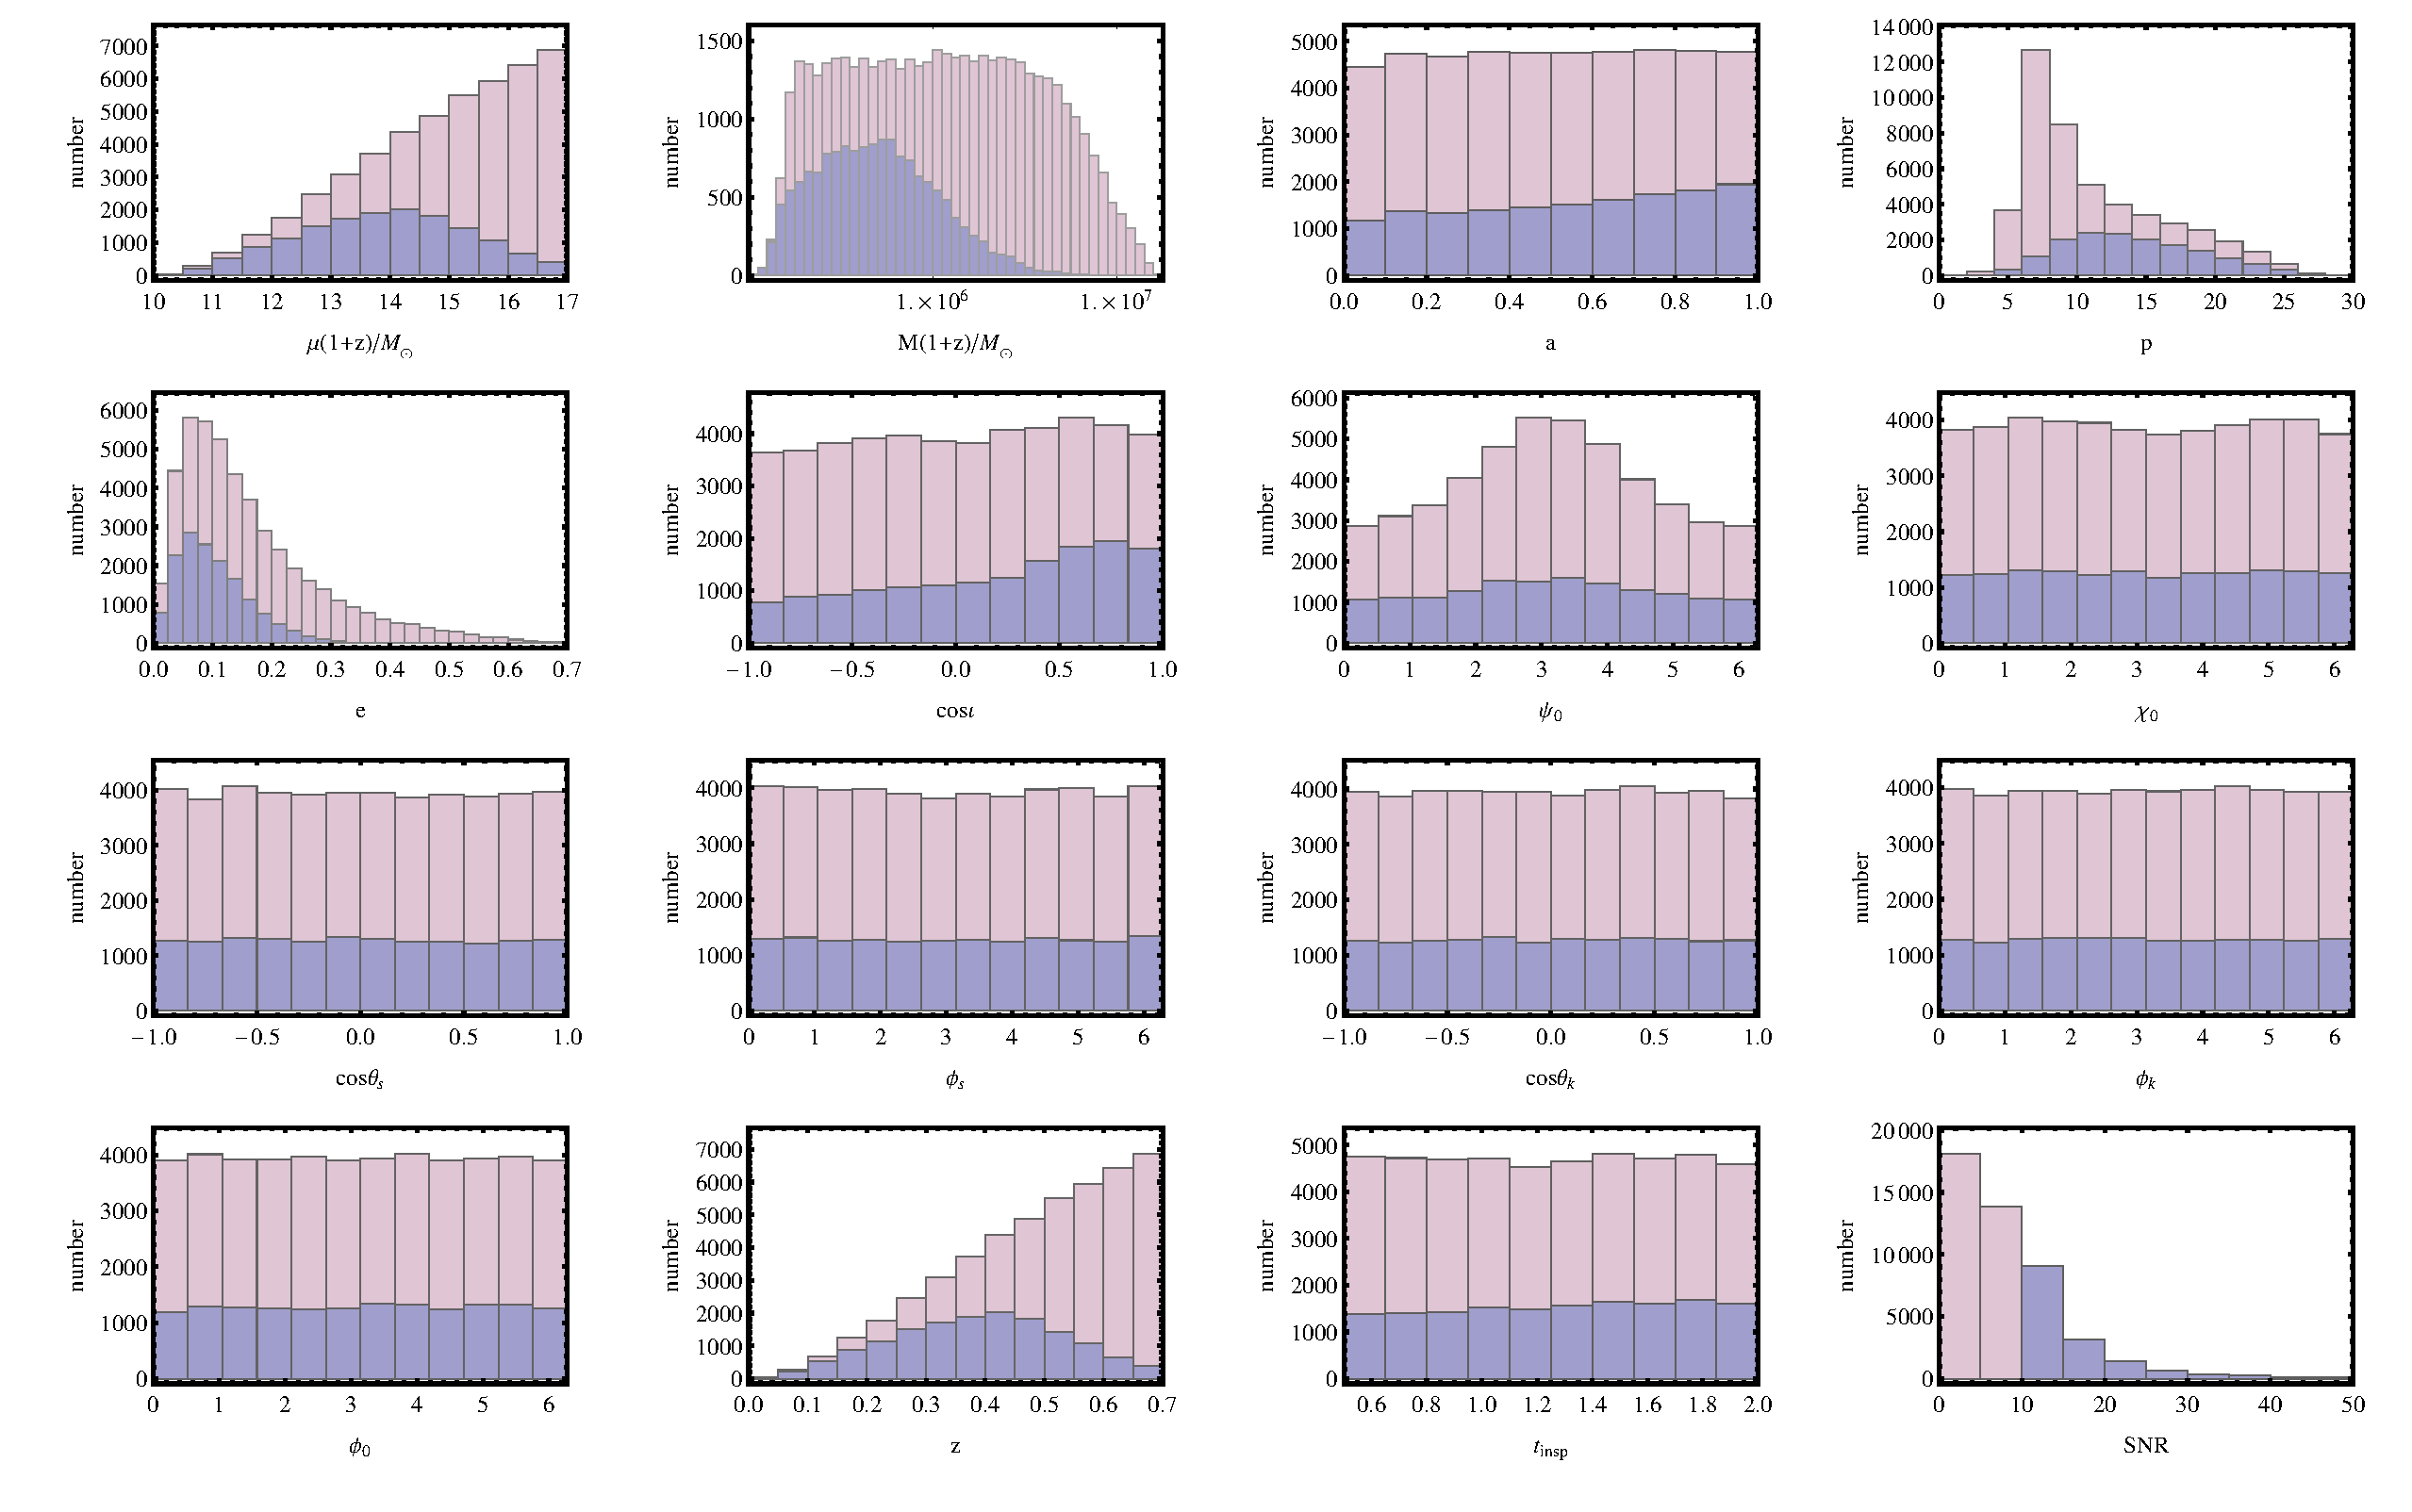
\includegraphics[width=\textwidth]{Fig_EMRIpar_dists}
\caption{\label{fig:EMRIpar-dists}The parameter distributions for our detectable EMRI systems, generated using $\mathcal{O}(10^4)$ realisations. The (darker) blue bars represent the final distribution, including an SNR cut of 10. The (lighter) pink bars stacked on top indicate the full distribution before the SNR cut.}
\end{figure*}

\subsection{Population results}
\label{sec:population}

\emph{THIS IS ALL GARBAGE (oh :()}

We take draws from the EMRI parameter distributions, using them as initial conditions for the full instantaneous evolution, from which we generate a family of adiabatic evolutions, as discussed in \secref{SNRloss}. There are broadly three categories of system regarding the effect of resonances on the evolution:

\begin{enumerate}
\item No significant resonance jumps are observed, and all the adiabatic models agree with the full evolution reasonably well: the overlaps are typically larger than $0.9$. The models have overlaps less than $1$ since the adiabatic approach breaks down near the end of the inspiral.

\item At least one resonance jump can be observed (typically the 2:3 resonance), but the adiabatic models still produce large overlaps. Most of the SNR from a signal is accumulated near to the end of the inspiral, at which point there are few significant resonances.

\item At least one resonance jump can be observed, and all of our chosen adiabatic models have low overlaps with the full evolution. This does not rule out the possibility of adiabatic models existing that would produce a high overlap, but it is difficult to predict the combination of parameters that would achieve this.
\end{enumerate}

To ensure that our chosen adiabatics are reasonable estimates to maximise the overlap, we computed many adiabatic waveforms with regular values of $t_\mathrm{match}$ for one particular system; there can be large fluctuations in the overlap, but our chosen parameters perform at least averagely well.

Across the full population, of $140$ different realisations, we find that $77\%$ of systems pass through the 2:3 resonance within the later stages of inspiral. In addition, $99\%$ of the systems we studied encountered the 1:2 resonance. This suggests that transient resonances are an important consideration in the evolution of EMRIs.

While resonance jumps may in principle be as large as a few percent (see the example in \figref{resjump-vs-q}), this tends to only occur in high eccentricity systems. The typical size of any resonance jump within our astrophysical population is less than $0.01\%$, with many systems showing no visible changes through resonance. \Figref{pop-SNR-vs-jump} shows the distribution of computed resonance jumps in $E$ for our population, along with the corresponding loss of overlap. There is no observed trend with the size of the resonance jump, although this is not surprising given the small size of the jumps. The large scatter on the plot is due to our choice of adiabatic family; in each case, the quoted fractional SNR is a lower bound for the actual fractional SNR across the entire adiabatic model space.

\begin{figure*}[htbp]
\centering
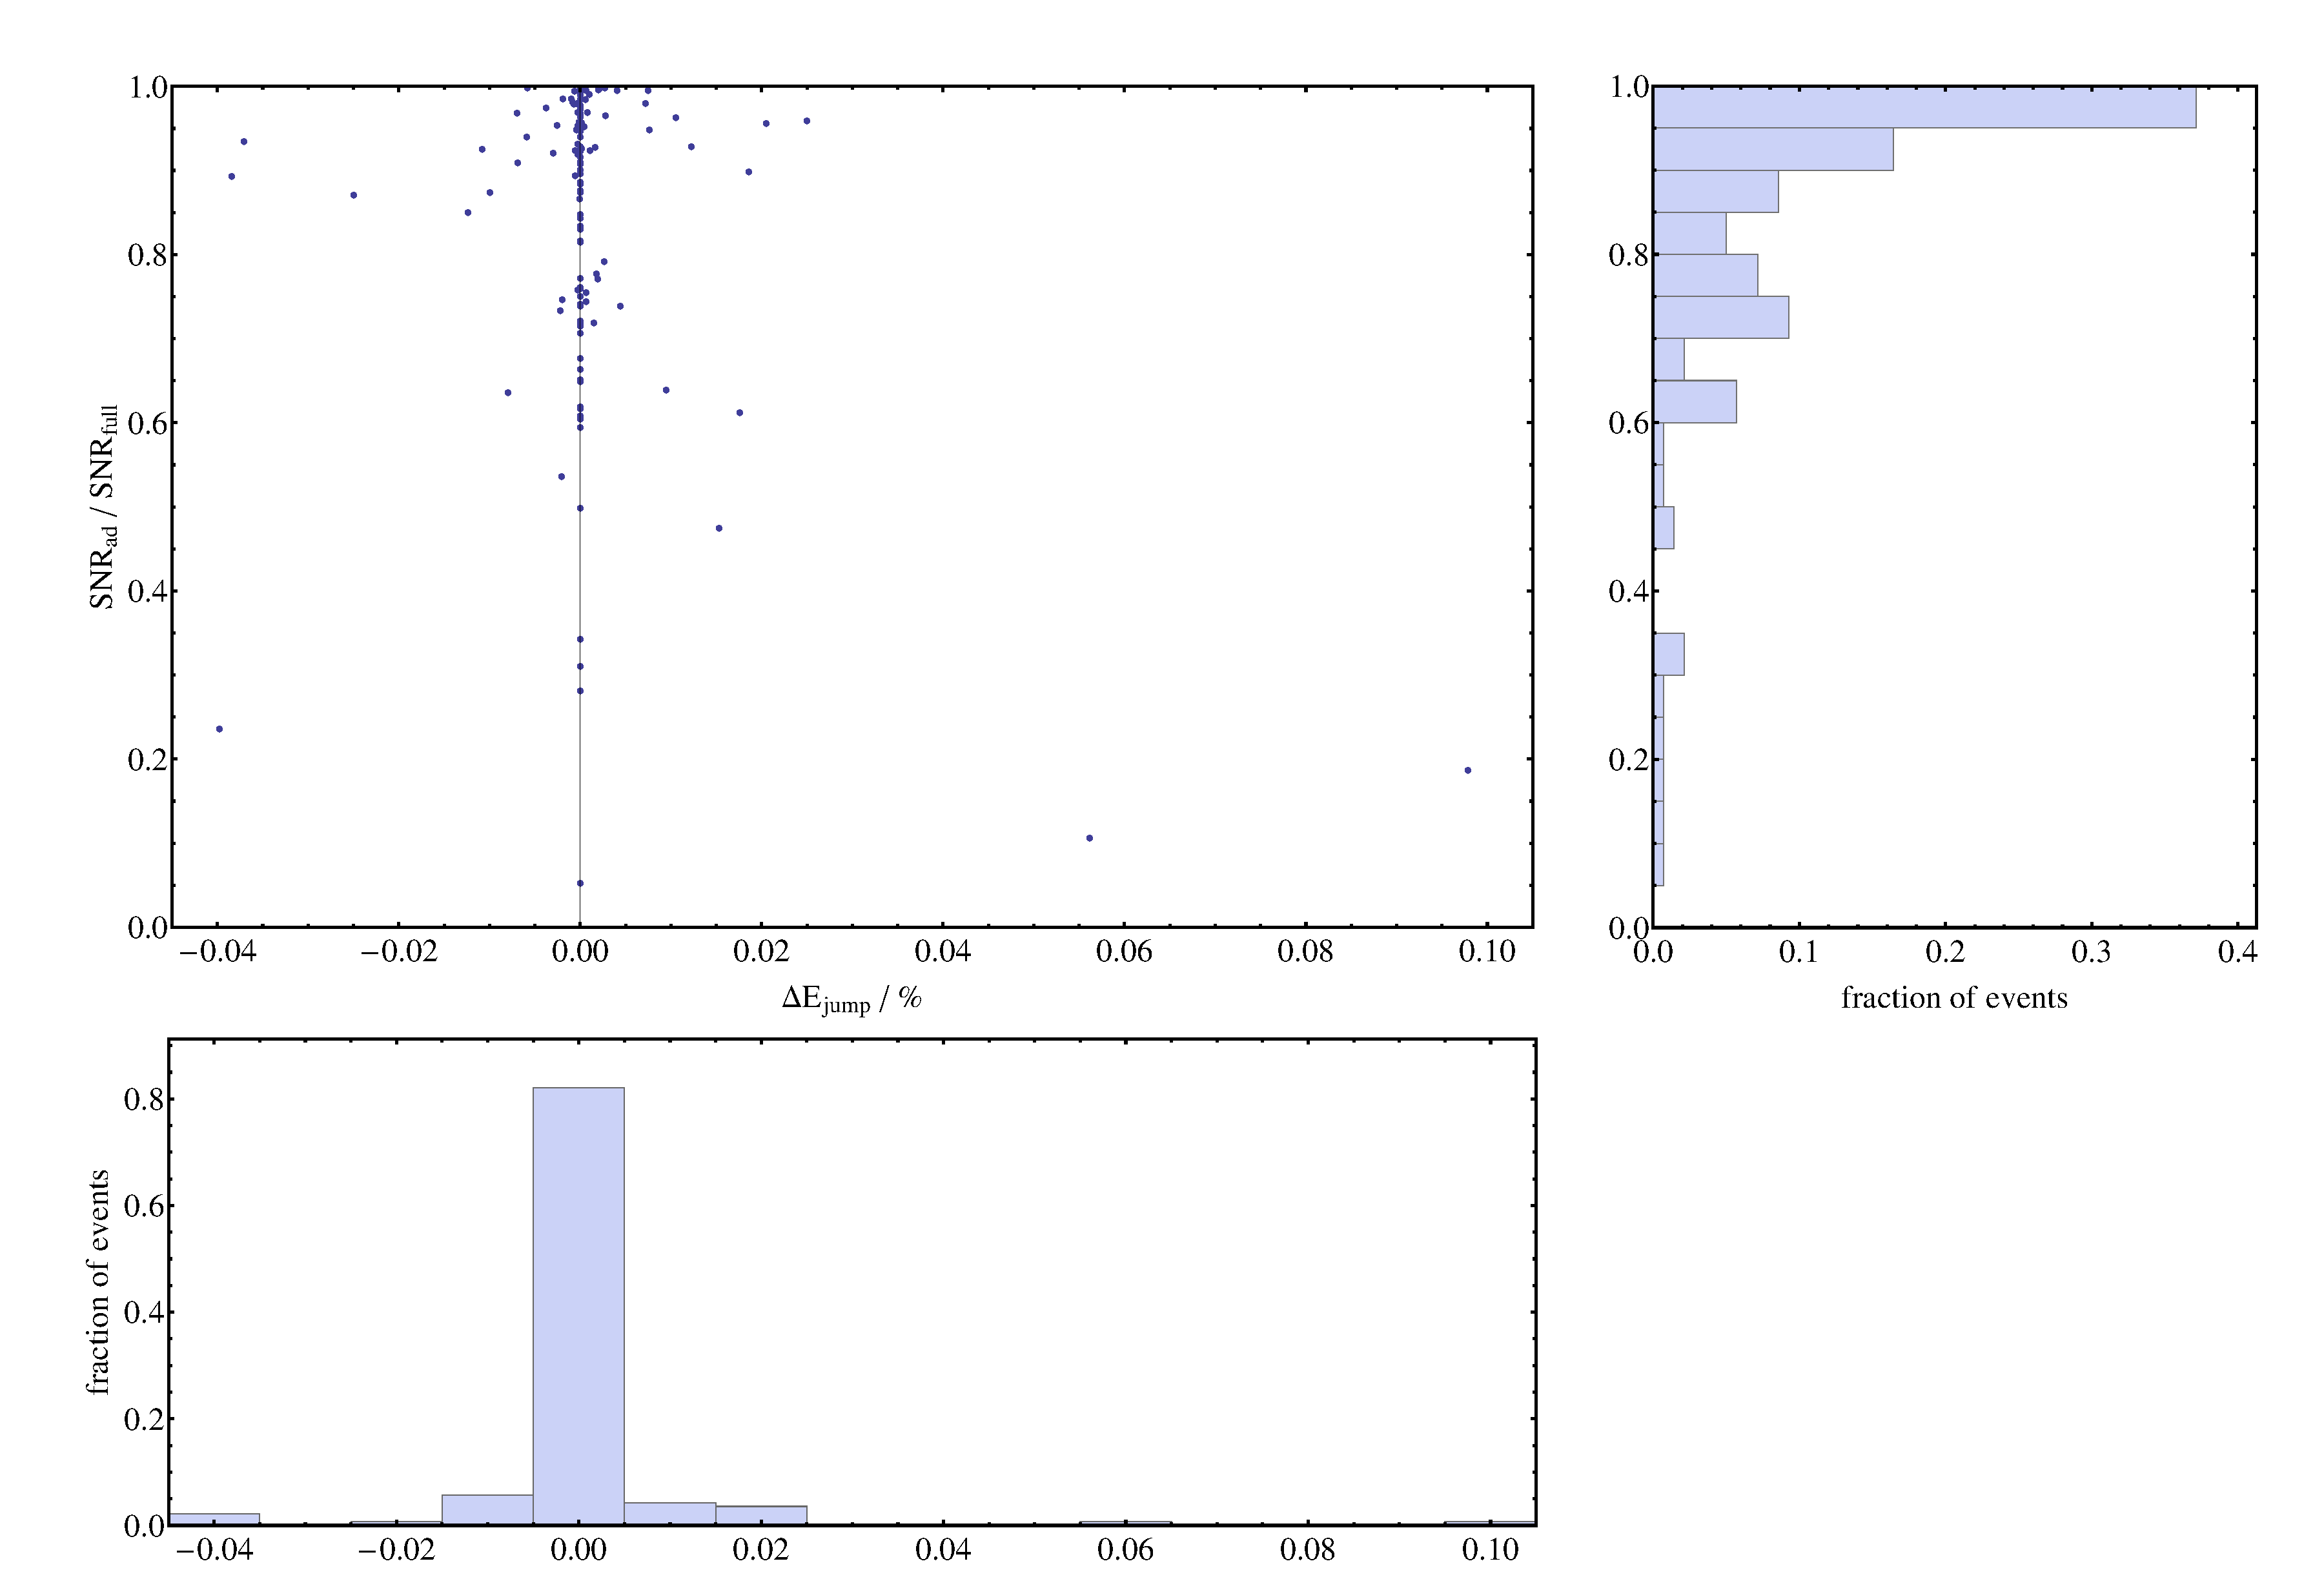
\includegraphics[width=0.92\textwidth]{Fig_pop_SNR_vs_jump}
\caption{\label{fig:pop-SNR-vs-jump}The fraction of the full SNR recovered using our family of adiabatic models, as a function of the percentage resonance jump in $E$. The histograms show the marginalised distributions over each parameter.}
\end{figure*}

It is possible for EMRIs to form through alternative channels, which may result in a population of high eccentricity systems. As an example, compact objects can be scattered onto orbits that plunge directly into the central BH; these systems can be mistaken for slow inspirals since they still undergo many hundreds of thousands of cycles in the bandwidth of a detector like eLISA \cite{Amaro-Seoane2013}. This kind of event is expected to be orders of magnitude more common than classic EMRIs. It is expected that resonance behaviours would be much more important in this case.

Even within the low eccentricity systems considered here, it is possible for some EMRIs to be undetectable using adiabatic models, given the resonances they encounter. These are any systems for which the full SNR is larger than some cutoff value, but the largest adiabatic SNR is smaller than the cutoff. The estimated fraction of systems that would be lost in this manner, as a function of cutoff SNR is shown in \figref{SNRcutoff}.

\begin{figure}[htbp]
\centering
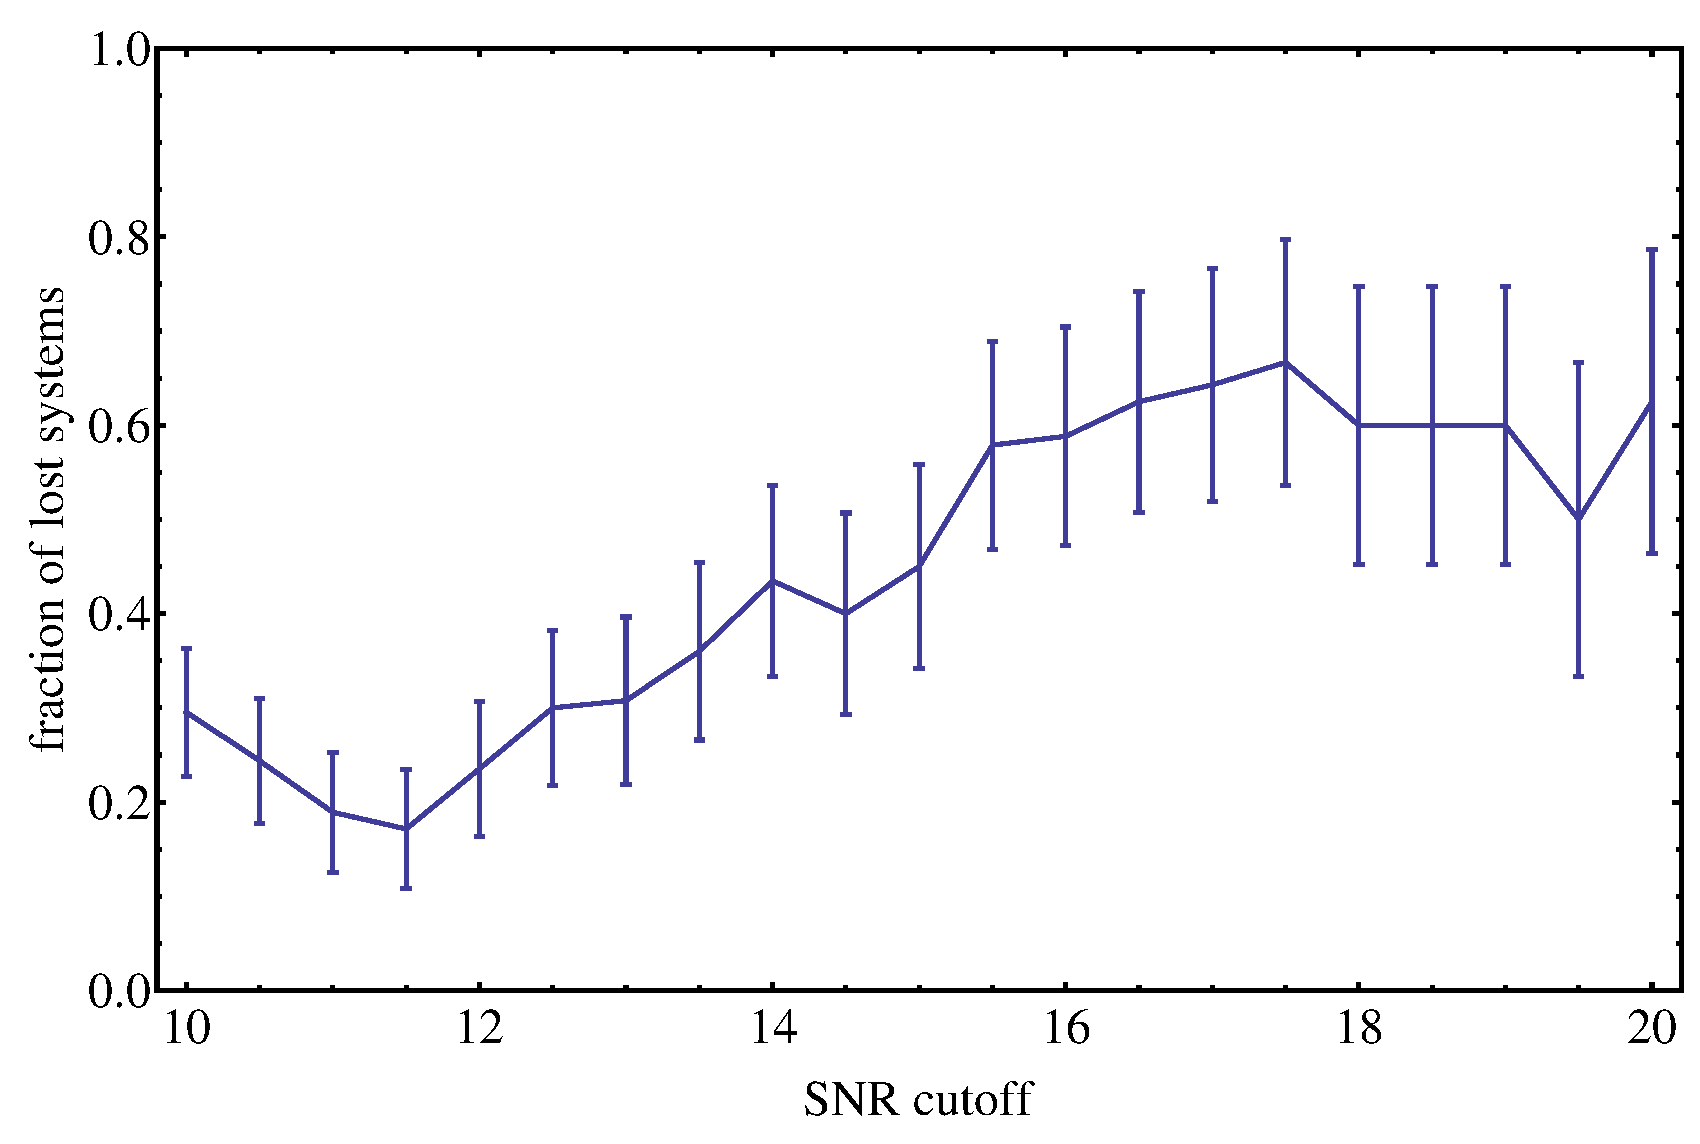
\includegraphics[width=0.46\textwidth]{Fig_SNRcutoff}
\caption{\label{fig:SNRcutoff}The fraction of EMRI systems that would be lost using adiabatic models to analyse data that contain the effects of transient resonances. The error bars are estimated using the beta distribution \cite{Cameron2011}.}
\end{figure}

\section{Concluding remarks}
\label{sec:conclusion}

\emph{Need to reconclude}

Transient resonances in EMRIs are an important consideration in waveform modelling due to the high proportion of expected systems encountering a low-order resonance in the later stages of inspiral. We have presented an evolution scheme appropriate for studying the effects of resonances on inspirals, which has been applied to an astrophysically realistic population. The location and duration of resonances, as well as their effect on orbital parameters, can all be calculated.

Amongst a population of sources, unmodelled resonances could diminish detection prospects. However, due to the low eccentricity of detectable sources, the overall effect on SNR recovery is small; it is therefore likely to be sufficient to use adiabatic models to detect EMRIs. An unresolved question here is how using these adiabatic models would affect parameter estimation: systematic biases may be introduced if we neglect the presence of important resonances. One method of providing an answer to this problem is to perform an MCMC parameter estimation study using our adiabatic waveforms as templates; we leave this to future work.

High eccentricity EMRIs may be possible, in which case transient resonances will play an important role in their detectability; systems that undergo a jump of a few percent dephase very rapidly from the adiabatic approximation. In such scenarios, adiabatic models can still be used, but there must be sufficient SNR in each non-resonant region that they can be detected as individual sources and then identified as arising from the same inspiral. If this is not possible, \eqnref{delta-I-a} can be used to join together different adiabatic models, if the phase on resonance and the magnitude of the self-force can be predicted sufficiently accurately. Alternatively, the jump $\Delta\mathcal{I}_\mathrm{jump}$ for each orbital parameter could be included as a free parameter in the template space, and then searched over. Such hybrid models merit further study as relatively simple ways of incorporating resonance effects into adiabatic models.

This work is highly dependent on the chosen self-force model, and so the results should be taken as qualitative estimates, given the unsuitability of a PN self-force to the problem of fast motion near to highly-spinning BHs. In the future, with a more accurate self-force model, more exact quantitative results can be derived.

\begin{acknowledgments}
The authors extend our sincere gratitude to \'{E}anna Flanagan and Tanja Hinderer for providing their PN self-force code, without which this work would not be possible. We also wish to thank Tanja Hinderer, Jeandrew Brink, Maarten van de Meent and Leor Barack for useful conversations. RHC is supported by STFC; CPLB was supported by STFC and the Cambridge Philosophical Society; PC is supported by a Marie Curie Fellowship, and JRG is supported by the Royal Society.
\end{acknowledgments}

\appendix

\section{Location of resonances}\label{sec:location}

We can find the location of resonances by numerically solving $\Omega = n_r \Omega_r - n_\theta \Omega_\theta = 0$. \Figref{res-plane-2-5-95} shows the semilatus rectum, eccentricity and (cosine of the) inclination angle of the $\nu = 2/5$ resonance surface for a BH of spin $a_\ast = 0.95$. 
\begin{figure}[htbp]
\centering
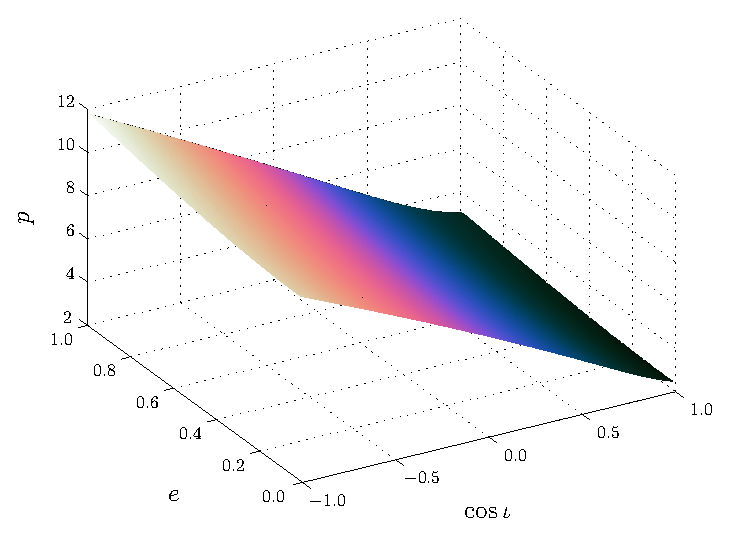
\includegraphics[width=0.46\textwidth]{Fig_res-2-5-95-plane}
\caption{\label{fig:res-plane-2-5-95}Location of the $2/5$ resonance surface for an $a_\ast = 0.95$ BH in terms of orbital semilatus rectum $p$, eccentricity $e$ and inclination $\iota$.}
\end{figure}
This is almost planar, inspiring us to look for a simple description that can help guide our search for resonance locations. Brink, Geyer and Hinderer~\cite{Brink2013} provide series expansions for the location of resonances in the limit of equatorial orbits for small spin and eccentricity. We do not follow this approach of trying to find analytic expressions for the resonance surface. The expressions become complicated when venturing away from limiting cases. Instead, we build an approximate phenomenological model and fit this to the resonance plane. %\footnote{A stopped clock is precisely correct twice a day, while a clock that is five minutes slow is never right but will often be close enough. Within this metaphor, our approximation would be a clock that varies between telling the correct time and being fifteen minutes off throughout the day: it is generally going to be good enough to give you a sense of the time but if you have an important event you should check with something better.}
This should be useful for designating the region in which resonance could be expected. To locate them precisely, it is necessary to solve $\Omega = 0$ numerically; the approximate model gives a suitable starting point.

The resonant semilatus rectum for any particular spin and resonance ratio can be well approximated as
\begin{equation}
p(e,\iota;a_\ast,\nu) \simeq A\frac{1 + B e + D \cos\iota}{1 - C\exp(e)}.
\end{equation}
The coefficients $\{A,B,C,D\}$ depend upon the spin and the particular resonance; they can be approximated as
\begin{align} 
A(a_\ast,\nu) \simeq {} & a_0\frac{1 + a_1\nu - a_2 \nu^2 - a_3 \nu a_\ast^2}{1 + a_4\nu - (1 + a_4)\nu^2}, \\
B(a_\ast,\nu) \simeq {} & b_0(1 - b_1\nu)\exp(-b_2\nu)(1 - b_3 a_\ast), \\
C(a_\ast,\nu) \simeq {} & c_0, \\
D(a_\ast,\nu) \simeq {} & d_0\left[1 - \exp(a_\ast)\right]\left[1 - d_1\exp(\nu)\right].
\end{align}
This gives us a total of $12$ parameters for our fit. Whilst this may sound large, if we were fitting an expansion to quadratic order in any combination of $\{e,\iota,a_\ast,\nu\}$ we would have $15$ parameters.\footnote{This does not give as good a fit as our function.} Our optimised parameters are
\begin{equation}
\begin{array}{lll}
a_0 = 5.9854, & a_1 = 3.4116, & a_2 = 0.9253,\\
a_3 = 0.1959, & a_4 = 4.8846, & b_0 = 0.7692,\\
b_1 = 1.4752, & b_2 = 1.4861, & b_3 = 0.5974,\\
c_0 = 0.02332, & d_0 = 0.7968, & d_1 = 0.3115.
\end{array}
\end{equation}
These were fitted for all possible resonances with $n_r = 2$--$7$ as well as $\nu = 9/10$, $19/20$, $49/50$ and $99/100$; with MBH spins of $a_\ast = 0.01$--$0.999$; for orbits with eccentricities $e = 0.01$--$0.99$, and inclinations $\cos\iota = -0.999999$--$0.999999$. 
%These were fitted for resonances with $\nu = 1/7, 1/6, 1/5, 1/4, 2/7, 1/3, 2/5, 3/7, 1/2, 4/7, 3/5, 2/3, 5/7, 3/4, 4/5, 5/6, 6/7, 9/10, 19/20, 49/50, 99/100$, with BH spins of $a_\ast = 0.01, 0.05, 0.1, 0.2, 0.3, 0.4, 0.5, 0.6, 0.7, 0.8, 0.9, 0.93, 0.95, 0.97, 0.99, 0.999$.
 
Using this approximation, the maximum error in $p$ for a given $a_\ast$ and $\nu$ is typically $\sim10\%$ and less that $1$ in absolute terms. The relative error in the semilatus rectum is illustrated in \figref{p-error}. 
\begin{figure*}[htp]
\centering
\centerline{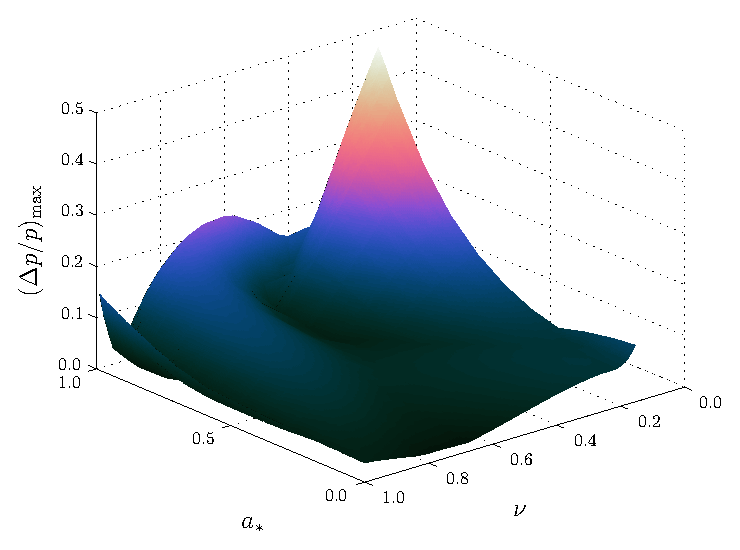
\includegraphics[width=0.47\textwidth]{Fig_fit-error-max-plane}\quad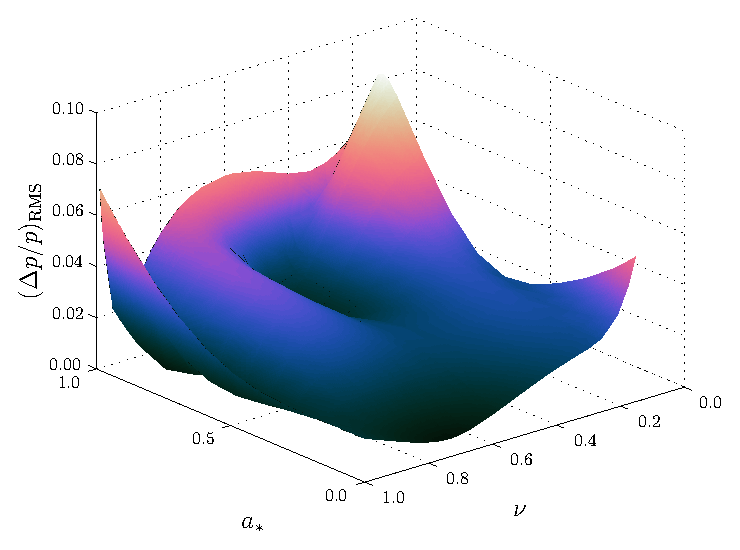
\includegraphics[width=0.47\textwidth]{Fig_fit-error-RMS-plane}}
\caption{\label{fig:p-error}Relative error in the approximate semilatus rectum compared to the accurate numerical result as a function of BH spin $a_\ast$ and resonance ratio $\nu$. The left panel shows the maximum relative error and the right shows the root-mean-square error; in both cases we are marginalising over eccentricity and inclination.}
\end{figure*}
The largest fractional error is $\sim50\%$, this is for $a\rightarrow 1$ and $\nu \rightarrow 0$, and corresponds to small $p$, such that the absolute error is still small. Taking the root-mean-square across $e$ and $\iota$, the fractional error for a given $a_\ast$ and $\nu$ never exceeds $9\%$ and is typically less than $4\%$.

\section{Asymptotic solution for passage through resonance}\label{sec:res-asymptotic}


The impact of passing through resonance on the evolution can be modelled analytically using asymptotic expansions~\cite{Gair2012}. Solutions for the motion are constructed far away from resonance and these are matched to a transition region in the vicinity of resonance~\cite{Kevorkian1971,Bosley1992}. By comparing the matched solution, which incorporates the effects of resonance, with the results of an adiabatic evolution, it is possible to estimate the discrepancy in the orbital parameters. This determines the difference in the orbital phase between the two approaches. If this error is sufficiently small, then it is safe to ignore the effects of the resonance; however, only a small difference is needed to impact the subsequent waveform, since the error accumulates over the subsequent observation of $\sim \order{\eta^{-1}}$ cycles~\cite{Flanagan2012}. We derive formulae which can be used to calculate the discrepancy in the orbital parameters.

The following derivation is reproduced from Berry~\cite{BerryThesis2013}. It is is based upon the analysis of Kevorkian~\cite{Kevorkian1987}; small adjustments have been made to adapt to the specific problem of GW inspiral, but the general argument is unchanged.\footnote{The same two time-scale theory underpins the analysis of Hinderer and Flanagan~\cite{Hinderer2008}, but this explicitly ignores resonances.} A similar derivation can be found by van de Meent~\cite{VanDeMeent2014}.

We model the system using action--angle variables. We are only concerned with the $r$ and $\theta$ motions, so we have a $2$-dimensional system. We perform a canonical transformation  to isolate the resonant combination $q = n_r q_r - n_\theta q_\theta$~\cite{Bosley1992,VanDeMeent2014}. This becomes one of the new angle variables, the other variable $q'$ can be either $q_r$ or $q_\theta$ (as, on resonance, varying one necessarily changes the other). We use $J$ as the conjugate action variable to $q$ and $\omega = n_r \omega_r - n_\theta \omega_\theta$ as its frequency. Similarly, we use $J'$ as the action variable conjugate to $q'$. The system evolves through resonance slowly, on an evolution time-scale, so we parameterize it in terms of a slow time parameter
\begin{equation}
\widetilde{\lambda} = \eta\lambda.
\end{equation}
The orbits of $q'$ proceed with the fast time $\lambda$; since this is much more rapid than the evolution we are interested in, it is safe to average over it. We are not interested in the fine-grained fast oscillations caused by changes in $q'$. For this analysis we consider the reduced problem of evolving $q$ and $J$.

At resonance $\widetilde{\lambda} = \widetilde{\lambda}_\star$ and $\omega\left(\widetilde{\lambda}_\star\right) = 0$. We assume that the frequency has a simple zero and can be expanded as
\begin{equation}
\omega\left(\widetilde{\lambda}\right) = \varpi_1\left(\widetilde{\lambda} - \widetilde{\lambda}_\star\right) + \varpi_2\left(\widetilde{\lambda} - \widetilde{\lambda}_\star\right)^2 + \ldots
\label{eq:omega-series}
\end{equation}
The frequency is actually a function of the angle variables, but since these evolve with $\widetilde{\lambda}$ it is safe to write it as a function of the slow time.\footnote{In effect we are defining $\omega\left(\tilde{\lambda}\right) \equiv \omega\left[J\left(\tilde{\lambda}\right)\right]$.}

Using the slow time, the equations of motion (\ref{eq:Mino-E-o-M}) become
\begin{subequations}
\begin{align}
\diff{q}{\widetilde{\lambda}} = {} & \dfrac{\omega(J)}{\eta} + \sum_s g_s^{(1)}(J)\exp(is q)  + \order{\eta}, \\
\diff{J}{\widetilde{\lambda}} = {} & \sum_s G_s^{(1)}(J)\exp(is q) + \order{\eta},
\end{align}
\end{subequations}
where we have rewritten the forcing terms as Fourier series and adapted the forcing functions to those appropriate for $q$ and $J$. We shall solve these before resonance and then match to solutions in the transition regime about resonance.

\subsection{Solution before resonance}\label{sec:before-res}

To find a solution away from the resonance, we decompose the problem to be a function of two time-scales~\cite{Kevorkian1971}. We use the slow time $\widetilde{\lambda}$ and, as a proxy for the fast time,
\begin{equation}
\Psi = \intd{0}{\lambda}{\omega(\eta\tau)}{\tau} = \recip{\eta}\intd{0}{\tilde{\lambda}}{\omega(\widetilde{\tau})}{\widetilde{\tau}}.
\end{equation}
From this
\begin{equation}
\omega = \diff{\Psi}{\lambda}.
\end{equation}
In terms of these two variables, we can build ansatz solutions
\begin{subequations}
\begin{align}
\label{eq:q-series}
q(\lambda;\,\eta) = {} & \Psi + q_0\left(\widetilde{\lambda}\right) + \eta q_1\left(\Psi,\widetilde{\lambda}\right) + \order{\eta^2}, \\
J(\lambda;\,\eta) = {} & J_0\left(\widetilde{\lambda}\right) + \eta J_1\left(\Psi,\widetilde{\lambda}\right) + \order{\eta^2}.
\label{eq:J-series}
\end{align}
\end{subequations}
We can also write a series expansion for the frequency, since it is affected by the self-force too,
\begin{equation}
\omega(\lambda;\,\eta) = \omega_0\left(\widetilde{\lambda}\right) + \eta \omega_1\left(\widetilde{\lambda}\right) + \order{\eta^2}.
\end{equation}
In the limit of $\eta \rightarrow 0$ we are left with a constant frequency $\omega_0(0)$. The higher-order terms are identified below by matching terms in the series expansions of the equations of motion. Taking the two time-scales as independent, we may write the time derivative to $\order{\eta}$ as
\begin{equation}
\diffop{\lambda} = \omega_0\partialdiffop{\Psi} + \eta\omega_1\partialdiffop{\Psi} + \eta\partialdiffop{\widetilde{\lambda}}.
\end{equation}

Using the two time-scale decomposition to replace the time derivatives in the equations of motion, and substituting in the ansatz expansions gives, to first order,
\begin{widetext}
\begin{subequations}
\begin{align}
\label{eq:q-1}
\omega_0 + \eta\omega_1 + \eta\partialdiff{q_0}{\widetilde{\lambda}} + \eta\omega_0\partialdiff{q_1}{\Psi} = {} & \omega(J_0) + \eta\diff{\omega}{J}J_1 + \eta \sum_s g_s^{(1)}(J_0)\exp\left[is(\Psi + q_0)\right], \\
\eta\partialdiff{J_0}{\widetilde{\lambda}} + \eta\omega_0\partialdiff{J_1}{\Psi} = {} & \eta \sum_s G_s^{(1)}(J_0)\exp\left[is(\Psi + q_0)\right].
\label{eq:J-1}
\end{align}
\end{subequations}
\end{widetext}
Averaging \eqnref{J-1} over $\Psi$ gives\footnote{The ansatz is constructed such that $J_0 \equiv \langle J_0\rangle_\Psi$ and $q_0 \equiv \langle q_0\rangle_\Psi$.}
\begin{equation}
\partialdiff{J_0}{\widetilde{\lambda}} = G_0^{(1)}(J_0).
\label{eq:J-ad}
\end{equation}
This describes the adiabatic evolution, hence we can identify $J_0\left(\widetilde{\lambda}\right)$ with (the lowest order piece of) the adiabatic solution~\cite{Hinderer2008}. If we similarly average \eqnref{q-1}, we find
\begin{equation}
\omega_0 + \eta\omega_1 +\eta\partialdiff{q_0}{\widetilde{\lambda}} = \omega(J_0) + \eta\partialdiff{\omega}{J}\langle J_1\rangle_\Psi + \eta g_0^{(1)}(J_0).
\end{equation}
From this we can identify the terms that originate from the frequency and, matching by order in $\eta$, obtain
\begin{subequations}
\begin{align}
\omega_0 = {} & \omega(J_0), \\
\omega_1 = {} & \partialdiff{\omega}{J}\langle J_1\rangle_\Psi.
\end{align}
\end{subequations}
This leaves
\begin{align}
\partialdiff{q_0}{\widetilde{\lambda}} = {} & g_0^{(1)}(J_0), \\
q_0 = {} & \kappa_0 + \intd{0}{\tilde{\lambda}}{g_0^{(1)}[J_0(\tau)]}{\tau}.
\label{eq:q-0-sol}
\end{align}
We now have expressions for the lowest order terms in the expansions.

Subtracting the $s = 0$ components from \eqnref{J-1} leaves
\begin{equation}
\omega_0\partialdiff{J_1}{\Psi} = \sum_{s\,\neq\,0} G_s^{(1)}(J_0)\exp\left[is(\Psi + q_0)\right].
\end{equation}
This can be solved to give
\begin{equation}
J_1 = \langle J_1\rangle_\Psi + \recip{\omega_0}\sum_{s\,\neq\,0} \dfrac{G_s^{(1)}(J_0)\exp\left[is(\Psi + q_0)\right]}{is}.
\label{eq:J-1-sol}
\end{equation}
We can do the same for \eqnref{q-1} to obtain
\begin{equation}
q_1 = \langle q_1\rangle_\Psi + \recip{\omega_0}\sum_{s\,\neq\,0} \dfrac{g_s^{(1)}(J_0)\exp\left[is(\Psi + q_0)\right]}{is}.
\label{eq:q-1-sol}
\end{equation}
To find the constants of integration, $\langle q_1\rangle_\Psi$ and $\langle J_1\rangle_\Psi$, it is necessary to extend the analysis to second order in $\eta$. This shows that $\langle J_1\rangle_\Psi$ is the first-order component of the adiabatic solution. We do not need explicit forms for later calculations, so we will not proceed further. We have successfully constructed the pre-resonance solution.

\subsection{Solution near resonance}\label{sec:interior-res}

Near to resonance, we consider an interior layer expansion~\cite{Kevorkian1971}. As explained in \secref{res-time}, evolution near resonance proceeds on a time-scale intermediate between the slow and fast times. We therefore introduce a rescaled time
\begin{equation}
\widehat{\lambda} = \dfrac{\widetilde{\lambda} - \widetilde{\lambda}_\star}{\eta^{1/2}} = \eta^{1/2}(\lambda - \lambda_\star).
\end{equation}
As for the before resonance solution, we can create a series expansion; however, now we expand in terms of $\eta^{1/2}$~\cite{Flanagan2012}
\begin{subequations}
\begin{align}
q\left(\widehat{\lambda};\,\eta\right) = {} & \widehat{q}_0\left(\widehat{\lambda}\right) + \eta^{1/2} \widehat{q}_{1/2}\left(\widehat{\lambda}\right) + \order{\eta}, \\
J\left(\widehat{\lambda};\,\eta\right) = {} & \widehat{J}_0 + \eta^{1/2} \widehat{J}_1\left(\widehat{\lambda}\right) + \order{\eta}.
\end{align}
\end{subequations}
The series expansion for the frequency, \eqnref{omega-series}, can be rewritten as
\begin{equation}
\omega\left(\widehat{\lambda}\right) = \eta^{1/2}\varpi_1\widehat{\lambda} + \eta\varpi_2\widehat{\lambda}^2 + \order{\eta^{3/2}}.
\label{eq:omega-hat}
\end{equation}
Proceeding to write the equations of motion in terms of the rescaled time gives
\begin{subequations}
\begin{align}
\diff{q}{\widehat{\lambda}} = {} & \varpi_1\widehat{\lambda} + \eta^{1/2}\varpi_2\widehat{\lambda}^2 \nonumber \\ 
 {} & + \left. \eta^{1/2}\sum_s g_s^{(1)}\left(\widehat{J}_0,\widetilde{\lambda}_\star\right)\exp(is \widehat{q}_0)  + \order{\eta}, \right. \\
\diff{J}{\widehat{\lambda}} = {} & \eta^{1/2}\sum_s G_s^{(1)}\left(\widehat{J}_0,\widetilde{\lambda}_\star\right)\exp(is \widehat{q}_0) + \order{\eta}.
\end{align}
\end{subequations}

From the equations of motion we can match terms by their order in $\eta^{1/2}$. At zeroth order we find
\begin{equation}
\widehat{J}_0 = \widehat{\varrho}_0
\end{equation}
is constant, and
\begin{equation}
\widehat{q}_0 = \widehat{\kappa}_0 + \dfrac{\varpi_1\widehat{\lambda}^2}{2}.
\end{equation}
Using these, we can build the next order terms
\begin{align}
\widehat{q}_{1/2} = {} & \widehat{\kappa}_{1/2} + \dfrac{\varpi_2\widehat{\lambda}^3}{3} + g_0^{(1)}(\widehat{\varrho}_0)\widehat{\lambda} \nonumber \\ 
 {} & + \sum_{s\,\neq\,0}g_s^{(1)}(\widehat{\varrho}_0)\exp(is \widehat{\kappa}_0)\intd{0}{\hat{\lambda}}{\exp\left(\dfrac{is \varpi_1\tau^2}{2}\right)}{\tau}, \\
\widehat{J}_{1/2} = {} & \widehat{\varrho}_{1/2} + G_0^{(1)}(\widehat{\varrho}_0)\widehat{\lambda} \nonumber \\
 {} & + \sum_{s\,\neq\,0}G_s^{(1)}(\widehat{\varrho}_0)\exp(is \widehat{\kappa}_0)\intd{0}{\hat{\lambda}}{\exp\left(\dfrac{is \varpi_1\tau^2}{2}\right)}{\tau}.
\end{align}
Both of these involve the complex Fresnel integral~\cite{Olver2010}, the details of which are given in the following section. We have now constructed the interior solution. % chapter 7

\subsection{The complex Fresnel integral}

The solution for the motion in the interior region near to resonance involves the integral
\begin{equation}
W\left(\widehat{\lambda}\right) = \intd{0}{\hat{\lambda}}{\exp\left(\dfrac{is \varpi_1\tau^2}{2}\right)}{\tau}.
\end{equation}
The complex Fresnel integral is
\begin{equation}
\mathcal{Y}(z) = \intd{0}{z}{\exp\left(\dfrac{i\pi x^2}{2}\right)}{x} = \mathcal{C}(z) + i\mathcal{S}(z),
\end{equation}
where $\mathcal{C}(z)$ and $\mathcal{S}(z)$ are the cosine and sine Fresnel integrals~\cite{Olver2010}, and hence % [7.2.7, 7.2.8]
\begin{equation}
W\left(\widehat{\lambda}\right) = \sqrt{\dfrac{\pi}{s\varpi_1}}\mathcal{Y}\left(\sqrt{\dfrac{s\varpi_1}{\pi}}\widehat{\lambda}\right).
\end{equation}

We shall be interested in the asymptotic behaviour for $|\widehat{\lambda}| \rightarrow \infty$. The complex Fresnel integral has the limit~\cite{Olver2010} % [7.5.3, 7.5.4, 7.12.2, 7.12.3]
\begin{equation}
\lim_{|z|\,\rightarrow\,\infty} \mathcal{Y}(z) \sim \dfrac{\sgn z}{\sqrt{2}} \exp\left(\dfrac{i\pi}{4}\right) - \dfrac{i}{\pi z}\exp\left(-\dfrac{i\pi z^2}{2}\right),
\end{equation}
where 
\begin{equation}
\sgn z = \begin{cases}
1 & z > 0 \\
-1 & z < 0
\end{cases}\,.
\end{equation}
Hence,
\begin{align}
\lim_{|\widehat{\lambda}|\,\rightarrow\,\infty}W\left(\widehat{\lambda}\right) \sim {} & \dfrac{\sgn \widehat{\lambda}}{\sqrt{2}}\sqrt{\dfrac{\pi}{|s\varpi_1|}}\exp\left[\sgn(s\varpi_1)\dfrac{i\pi}{4}\right] \nonumber \\
  {} & + \recip{is\varpi_1}\exp\left(\dfrac{is \varpi_1 \widehat{\lambda}^2}{2}\right).
\label{eq:Fres-limit}
\end{align}

\subsection{Matching solutions}

To complete our solution we must match the pre-resonance solution of \secref{before-res} with the near resonance solution of \secref{interior-res}. This is achieved by rewriting the pre-resonance solution in terms of the rescaled time $\widehat{\lambda}$ and comparing this with the near resonance solution expanded in the limit of $\widehat{\lambda} \rightarrow -\infty$.

To rewrite the pre-resonance solution, we begin with the fast phase parameter
\begin{equation}
\Psi\left(\widehat{\lambda}\right) = \dfrac{\Psi_\star}{\eta} + \dfrac{\varpi_1\widehat{\lambda}^2}{2} + \eta^{1/2}\dfrac{\varpi_2\widehat{\lambda}^3}{3} + \order{\eta}.
\end{equation}
Using this together with equations (\ref{eq:q-0-sol}) and (\ref{eq:q-1-sol}) in \eqnref{q-series}, the angle variable is
\begin{widetext}
\begin{align}
q\left(\widehat{\lambda};\,\eta\right) = {} & \dfrac{\Psi_\star}{\eta} + \dfrac{\varpi_1\widehat{\lambda}^2}{2} + \kappa_\star + \eta^{1/2}\dfrac{\varpi_2\widehat{\lambda}^3}{3} + \eta^{1/2}g_0^{(1)}(J_\star)\widehat{\lambda} + \dfrac{\eta^{1/2}}{\varpi_1\widehat{\lambda}}\sum_{s\,\neq\,0}\recip{is}g_s^{(1)}(J_\star)\exp\left[is\left(\dfrac{\Psi_\star}{\eta} + \dfrac{\varpi_1\widehat{\lambda}^2}{2} + \kappa_\star\right)\right] + \order{\eta},
\end{align}
where we have defined $J_\star \equiv J_0\left(\widetilde{\lambda}_\star\right)$ and $\kappa_\star = \kappa_0 + \intd{0}{\tilde{\lambda}_\star}{g_0^{(1)}[J_0(\tau)]}{\tau}$, and used \eqnref{omega-hat} to substitute for $\omega$. The action variable is similarly determined by using equations (\ref{eq:J-ad}) and (\ref{eq:J-1-sol}) with \eqnref{J-series} to give
\begin{align}
J\left(\widehat{\lambda};\,\eta\right) = {} & J_\star + \eta^{1/2}G_0^{(1)}(J_\star)\widehat{\lambda} + \dfrac{\eta^{1/2}}{\varpi_1\widehat{\lambda}}\sum_{s\,\neq\,0}\recip{is}G_s^{(1)}(J_\star)\exp\left[is\left(\dfrac{\Psi_\star}{\eta} + \dfrac{\varpi_1\widehat{\lambda}^2}{2} + \kappa_\star\right)\right] + \order{\eta}.
\end{align}
\end{widetext}
We can now compare this to the near resonance expansion with the integral replaced by the limiting form given in \eqnref{Fres-limit}.

At zeroth order, we immediately obtain
\begin{align}
\widehat{\kappa}_0 = {} & \dfrac{\Psi_\star}{\eta} + \kappa_\star, \\
\widehat{\varrho}_0 = {} & J_\star.
\end{align}
These fix the integration constants. The more interesting result is now found by comparing the $\order{\eta^{1/2}}$ terms. Equating the angle variable expressions and cancelling terms gives
\begin{align}
%\widehat{\kappa}_{1/2} + \sum_{s\,\neq\,0}g_s^{(1)}(\widehat{\varrho}_0)\exp(is \widehat{\kappa}_0)\left\{\dfrac{\sgn \widehat{\lambda}}{\sqrt{2}}\sqrt{\dfrac{\pi}{|s\varpi_1}}\exp\left[\sgn(s\varpi_1)\dfrac{\pi}{4}\right] + \recip{is\varpi_1}\exp\left(\dfrac{is \varpi_1 \widehat{\lambda}^2}{2}\right)\right\} = {} & \recip{is\varpi_1\widehat{\lambda}}g_s^{(1)}(\widehat{\varrho}_0)\exp\left[is\left(\dfrac{\Psi_\star}{\eta} + \dfrac{\varpi_1\widehat{\lambda}^2}{2}\right)\right] \nonumber \\
\widehat{\kappa}_{1/2} = {} & \sum_{s\,\neq\,0}g_s^{(1)}(\widehat{\varrho}_0)\sqrt{\dfrac{\pi}{2|s\varpi_1|}}\exp\left[i\left(s \widehat{\kappa}_0 + \dfrac{\pi}{4}\sgn s\varpi_1\right)\right].
\end{align}
Similarly, for the action variables
\begin{equation}
\widehat{\varrho}_{1/2} = \sum_{s\,\neq\,0}G_s^{(1)}(\widehat{\varrho}_0)\sqrt{\dfrac{\pi}{2|s\varpi_1|}}\exp\left[i\left(s \widehat{\kappa}_0 + \dfrac{\pi}{4}\sgn s\varpi_1\right)\right].
\label{eq:J-1/2}
\end{equation}
We now have a matched solution through resonance.

Having constructed the solution, we see that the lowest order evolution corresponds to the adiabatic solution; the deviations come in at the following order. When we switch from the pre-resonance solution to the post-resonance solution, there is a change in the sign of $\widehat{\lambda}$. Therefore, when matching the post-resonance solution $\widehat{\varrho}_{1/2}$ and $\widehat{\kappa}_{1/2}$ also change sign: there is a change of
\begin{align}
\Delta q = {} & 2 \eta^{1/2}\widehat{\kappa}_{1/2}, \\
\Delta J = {} & 2 \eta^{1/2}\widehat{\varrho}_{1/2}
\label{eq:jumps}
\end{align}
across the resonance~\cite{Kevorkian1987}. We are not particularly interested in the deviation in $J$, of greater concern is the change in the orbital parameters $\{E,L_z,Q\}$. Assuming that there is a smooth transformation that maps between $J$ and these, then, to lowest order, we can calculate the deviation relative to the adiabatic prescription by substituting the forcing functions $G^{(1)} \rightarrow G_a^{(1)}$, where $G_a^{(1)}$ describes the evolution of $\mathcal{I}_a$ through the effects of the self-force. This result is quoted by Flanagan and Hinderer~\cite{Flanagan2012}. The change in the orbital parameters is determined by the forcing functions, hence it is essential to have an accurate self-force model.

As a final step in understanding our result, we switch from Mino time to coordinate time. An appropriate redefinition of the forcing functions can be done by scaling by $\Gamma$, we define
\begin{equation}
F_a^{(1)} = \dfrac{G_a^{(1)}}{\Gamma},
\end{equation}
such that the equation of motion becomes
\begin{equation}
\left\langle \diff{\mathcal{I}_a}{t}\right\rangle_{q'} =  \eta\sum_s F_{a,\,s}^{(1)}(\boldsymbol{\mathcal{I}})\exp(is q) + \order{\eta^2}.
\end{equation}
Here we have made the averaging over $q'$ explicit to show that the equation is only defined as an orbital average: not only does our asymptotic expansion average out oscillations over an orbit in $q'$, but in converting from $\lambda$ to $t$ we have used $\Gamma$ which is an orbital average.
From \eqnref{omega-series}, we recognise that
\begin{equation}
\varpi_1 = \partialdiff{\omega}{\widetilde{\lambda}} = \dfrac{\Gamma^2}{\eta}\left\langle\dot{\Omega}\right\rangle_{q'}.
\end{equation}
We have used the averaged form of $\dot{\Omega}(t)$ as this is appropriate. Using these to adapt equations (\ref{eq:J-1/2}) and (\ref{eq:jumps}), we obtain
\begin{align}
\Delta \mathcal{I}_a = {} & \eta\sum_{s\,\neq\,0}F_{a,\,s}^{(1)}(\boldsymbol{\mathcal{I}}_\star)\left[\dfrac{2\pi}{\left|s \left\langle\dot{\Omega}\right\rangle_{q'}\right|}\right]^{1/2} \nonumber \\*
 {} & \times \left.\exp\left[i\left(s \widehat{\kappa}_0 + \dfrac{\pi}{4}\sgn s\dot{\Omega}\right)\right]\right. \\
 = {} & \eta\sum_{s\,\neq\,0}F_{a,\,s}^{(1)}(\boldsymbol{\mathcal{I}}_\star)\tau_{\mathrm{res},\,s}\exp\left[i\left(s \widehat{\kappa}_0 + \dfrac{\pi}{4} \sgn s\dot{\Omega} \right)\right],
\end{align}
using \eqnref{T-res-s} and representing the values on resonance of $E$, $L_z$ and $Q$ with $\boldsymbol{\mathcal{I}}_\star$.


\bibliography{Resonances}

\end{document}
